\documentclass[11pt]{report}
\usepackage{graphicx}
\usepackage{sidecap}
\usepackage{hyperref}
\usepackage[margin=3cm]{geometry}
\usepackage{listings}
\usepackage{xcolor}
\usepackage{svg}
\usepackage{tikz}
\usepackage{amsmath}
\usepackage[backend=bibtex]{biblatex}
\usepackage[utf8]{inputenc}
\usepackage{pgfplots}
\usepackage{tikz}
\usepackage{circuitikz}
\usepackage{textcomp}
\usepackage{siunitx}
\usepackage[caption=false,font=normalsize,labelfont=sf,textfont=sf]{subfig}
\usepackage{stfloats}

\usetikzlibrary {arrows.meta,automata,positioning}

% Define colors
\definecolor{codegreen}{rgb}{0,0.6,0}
\definecolor{codeblue}{rgb}{0,0,0.8}
\definecolor{codepurple}{rgb}{0.58,0,0.82}
\definecolor{backcolour}{rgb}{0.95,0.95,0.92}

% Define listing style for Python
\lstdefinestyle{python}{
    backgroundcolor=\color{backcolour},   
    commentstyle=\color{codegreen},
    keywordstyle=\color{codeblue}\bfseries,
    numberstyle=\tiny\color{gray},
    stringstyle=\color{codepurple},
    basicstyle=\ttfamily\footnotesize,
    breakatwhitespace=false,         
    breaklines=true,                 
    captionpos=b,                    
    keepspaces=true,                 
    numbers=left,                    
    numbersep=5pt,                  
    showspaces=false,                
    showstringspaces=false,
    showtabs=false,                  
    tabsize=4
}

% Define colors
\definecolor{keywordcolor}{rgb}{0,0,0.8}
\definecolor{commentcolor}{rgb}{0,0.5,0}
\definecolor{stringcolor}{rgb}{0.58,0,0.82}
\definecolor{backgroundcolor}{rgb}{0.95,0.95,0.92}
\definecolor{numbercolor}{rgb}{0.5,0.5,0.5}

% Define Verilog listing style
\lstdefinestyle{verilog}{
    language=Verilog,
    backgroundcolor=\color{backgroundcolor},
    basicstyle=\ttfamily\footnotesize,
    keywordstyle=\color{keywordcolor}\bfseries,
    commentstyle=\color{commentcolor}\itshape,
    stringstyle=\color{stringcolor},
    numberstyle=\tiny\color{numbercolor},
    numbers=left,
    numbersep=5pt,
    breaklines=true,
    showstringspaces=false,
    tabsize=4
}

% Define Tcl listing style
\lstdefinestyle{tclstyle}{
    language=Tcl,
    basicstyle=\ttfamily\footnotesize,
    keywordstyle=\color{blue}\bfseries,
    commentstyle=\color{green!50!black}\itshape,
    stringstyle=\color{red},
    morekeywords={proc, set, if, else, foreach, while, expr, return, puts, global, namespace, variable, array, dict, switch, after, update, uplevel, upvar},
    numbers=left,
    numberstyle=\tiny\color{gray},
    stepnumber=1,
    numbersep=5pt,
    backgroundcolor=\color{gray!10},
    frame=single,
    breaklines=true,
    breakatwhitespace=true,
    tabsize=4,
    showstringspaces=false
}

\addbibresource{refs.bib}

\title{%
    Handwritten Digit Recognition Neural Network  \\
    \medskip \\
    \large Digital System Design Project \\
    \large University of Pisa}
\author{Leonardo Bove \\
        Alessandro Porta}
\date{February 2025}

\begin{document}

\maketitle
\newpage
\tableofcontents

\chapter{Introduction}  

This project aims to design, simulate, and implement a neural network on the Altera DE10-Lite FPGA board to recognize handwritten digits from a touchscreen. The primary objective is to develop a fully synchronous digital architecture using Verilog, ensuring efficient hardware implementation.  

The project begins with a Python-based neural network model to train the system off-line and generate the necessary parameters. Once the model is validated in software, a corresponding hardware implementation is developed using Verilog. A digital twin is created to simulate the neural network's behavior before synthesizing it on the FPGA.  

Beyond the core neural network implementation, a complete system architecture is designed, incorporating multiple subsystems. This includes a controller module responsible for managing data flow, a graphical interface for touchscreen and LCD interaction, and an intermediate subsystem to bridge these components seamlessly.  

The entire project is synthesized and analyzed using Quartus Prime Lite Edition 18.1, with considerations for timing constraints, resource utilization, and hardware fitting. Finally, the complete system is deployed on the DE10-Lite board, where it undergoes real-world testing. The results demonstrate a successfully functioning handwritten digit recognition system, capable of processing and displaying user-drawn digits in real time.  

The entire project can be found on \href{https://github.com/leonardobove/handwritten_digit_recognition}{GitHub}.

\section{Project Objectives}  

The main goal of this project is to design and implement a fully synchronous digital system that adheres to the principles of synchronous digital design, as described in \cite{wakerly2005digital}. The entire project is developed strictly using Verilog, without relying on SystemVerilog features. This constraint ensures a more hardware-oriented implementation, emphasizing low-level digital design techniques.  

The primary objective is to create a pre-trained neural network for handwritten digit recognition. This neural network interacts with a touchscreen, allowing a user to draw digits. The system processes the input, performs inference, and displays the predicted digit on a seven-segment display. The design integrates multiple subsystems, including touchscreen input handling, neural network computation, and display output, all controlled by a finite state machine (FSM) to ensure proper sequencing and synchronization.  

\section{Requirements}
This project was implemented on the \textbf{Altera 10M50DAF484C7G MAX10} FPGA, mounted on the Altera \textbf{DE10-Lite} development board. For the user input, the \textbf{Terasic LT24 LCD touch 2.4"} module was chosen. It is compatible with the DE10-Lite board, where it can be easily mounted on the GPIO header, as shown in Fig. \ref{fig:hw_preview}.

\begin{figure}[!h]
    \centering
    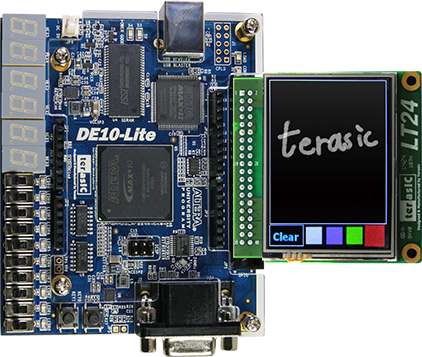
\includegraphics[width=0.5\linewidth]{images/introduction/hardware_preview.png}
    \caption{Hardware setup of the system.}
    \label{fig:hw_preview}
\end{figure}

The project was eventually synthesized, fitted and programmed on the device using \textbf{Quartus Prime Lite Edition 18.1}.


\chapter{System Architecture}
The whole system is comprised of three main blocks:

\begin{itemize}
    \item \textbf{Controller}: it implements the main finite-state machine of the system and controls the activation of the other slave finite-state machines.
    \item \textbf{Neural Network}: it implements the actual neural network that predicts the written digit based on the touchscreen input.
    \item \textbf{Graphic Interface}: it manages the drivers necessary to obtain the touchscreen input and to print on the LCD display what has been drawn by the user.
\end{itemize}

A simplified block schematic of the system is shown in Fig. \ref{fig:system_block_schem}.

\begin{figure}[!ht]
\centering
\resizebox{1\textwidth}{!}{%
\begin{circuitikz}
\tikzstyle{every node}=[font=\small]
\draw  (5,10.25) rectangle  node {\normalsize Controller} (8.75,7.75);
\draw  (1.25,5.25) rectangle  node {\normalsize Neural Network} (5,2.75);
\draw  (8.75,5.25) rectangle  node {\normalsize Graphic Interface} (12.5,2.75);
\draw [->, >=Stealth] (8.75,4) -- (5,4)node[pos=0.5,above, fill=white]{Touchscreen Data};
\draw [<->, >=Stealth, dashed] (12.5,4) -- (15,4);
\draw [->, >=Stealth, dashed] (2.5,9) -- (5,9)node[pos=0,left, fill=white]{Push-button inputs};
\draw [->, >=Stealth, dashed] (8.75,9) -- (11.25,9);
\draw [ dashed] (15,5.25) rectangle  node {\normalsize LT24 }  (17.5,2.75);
\draw [ dashed] (11.25,10.25) rectangle  node {\footnotesize Seven-segment display}  (15,7.75);
\draw [<->, >=Stealth] (5,7.75) -- (2.5,5.25)node[pos=0.5,undefined, fill=white]{Control Signals};
\draw [<->, >=Stealth] (8.75,7.75) -- (11.25,5.25)node[pos=0.5,undefined, fill=white]{Control Signals};
\draw [->, >=Stealth] (3.75,5.25) -- (6.25,7.75)node[pos=0.5,right, fill=white]{Predicted Digit};
\end{circuitikz}
}%
\caption{Schematic block view of the system.}
\label{fig:system_block_schem}
\end{figure}

In particular, each block was implemented using finite-state machines, which can be enabled and disabled by the main controller. Among the control signals shown in Fig. \ref{fig:system_block_schem}, enable, reset and status signals are present, which allow the controller to activate or deactivate the slave finite-state machines in precise moments and to manage the flow of data from the LT24 display up to the final seven-segment display output. The interface for each single sub-system will be explained in the next chapters.

This system was implemented on Quartus and the full block design is shown in Fig. \ref{fig:quartus_full_system}.

\begin{figure}[!ht]
    \centering
    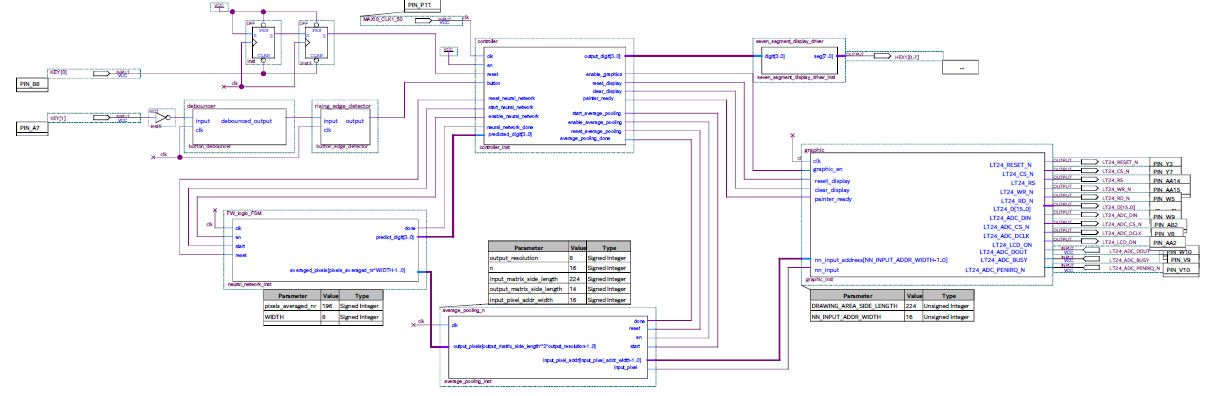
\includegraphics[width=1.0\linewidth]{images/system_architecture/quartus_full_system.png}
    \caption{Block design of the full system on Quartus.}
    \label{fig:quartus_full_system}
\end{figure}

In this Quartus block design, other sub-systems, such as the \textit{Average Pooling} and the \textit{Seven-segment Display Driver} are present, which will be better explained in Sec. \ref{sec:average_pooling} and \ref{sec:seven_segment_driver} respectively.

\section{Clock}
The global clock used for all the modules inside this design is the 50 MHz clock generated on the DE10-Lite board by the CDCE937 clock generator.

Where slower clock frequencies were necessary, an enable control technique was used, in order to guarantee a static synchronous design with a single clock domain: the state registers of these finite-state machines are still clocked at 50 MHz, but they are enabled only at every N clock cycles, where N is a power of 2. This solution is accomplished through an enable generator, which can be implemented with the following Verilog code:

\begin{lstlisting}[
language=Verilog,
style=verilog,
caption=Enable generator implementation.,
label= list:enable_generator]
module enable_generator #(
    parameter COUNTER_SIZE = 3
)(
    input input_clock,
    output output_enable
);
    reg [(COUNTER_SIZE-1):0] counter = 0;
    
    always @ (posedge input_clock)
        if (counter == (2**COUNTER_SIZE)-1) counter <= 0;
        else counter <= counter + 1'b1;

    assign output_enable = (counter == (2**COUNTER_SIZE)-1);
endmoduleput reg done // Done signal indicating completion
);
\end{lstlisting}


\chapter{Controller Design} 

\begin{figure}[!h]
    \centering
    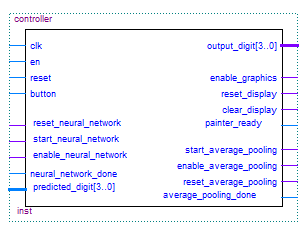
\includegraphics[width=0.6\linewidth]{images/controller/controller_quartus_block.png}
    \caption{Quartus block of Controller.}
    \label{fig:controller}
\end{figure}

The controller (shown in fig. \ref{fig:controller}) is the central module of the system, responsible for orchestrating the execution of different functional blocks. It implements a master finite state machine (FSM) that manages three slave FSMs: one handling the graphical interface, one controlling the neural network processing and the average pooling which acts as an intermediate processing stage between the neural network and the graphical interface. The controller ensures proper synchronization between these components, allowing efficient processing of input data and display of the final result.  

The main tasks of the controller include:  
\begin{itemize}  
    \item Managing the \textbf{graphics interface}, responsible for clearing and updating the display.  
    \item Controlling the \textbf{average pooling module}, which processes the input data before feeding it into the neural network.  
    \item Coordinating the \textbf{neural network module}, ensuring it starts execution at the appropriate time and retrieving the computed result.  
    \item Handling \textbf{push-button inputs}, ensuring they are correctly debounced and synchronized with the system clock.  
    \item Driving the \textbf{seven-segment display}, showing the final predicted digit once processing is complete.  
\end{itemize}  

This chapter is structured as follows: sec. \ref{sec:fsm_controller} describes the \textbf{finite state machine (FSM)} of the controller, explaining the different states and transitions governing the system's operation, sec. \ref{sec:push-button_inputs} discusses the \textbf{push-button inputs} and the logic used to ensure synchronization within a synchronous digital design and, finally, sec. \ref{sec:seven_segment_driver} details the \textbf{seven-segment display driver} and its role in visualizing the predicted output.   

\section{Finite-State Machine}
\label{sec:fsm_controller}

\begin{figure}[!h]
\centering
\resizebox{1\linewidth}{!}{% Reduce size of everything
\begin{tikzpicture}[shorten >=1pt, node distance=3cm, on grid,
                    initial distance=1cm, initial text=reset,
                    bend angle=45,
                    every state/.style={font=\footnotesize},
                     initial/.style ={font=\footnotesize}] 
    %\draw[help lines] (0,-5) grid (10,10);

   \node[] (reset_in) at (-4,4) {};

   \node[state] (reset) at (-2, 4) {RESET};
   \node[state, text width=2cm, align=center] (clear_display_start) {CLEAR DISPLAY START};
   \node[state, text width=2cm, align=center] (clear_display_wait) at (2,4) {CLEAR DISPLAY WAIT}; 
   \node[state] (idle) at (8,4) {IDLE}; 
   \node[state, text width=2cm, align=center] (average_pooling_start) at (14,4) {AVERAGE POOLING START};
   \node[state, text width=2cm, align=center] (average_pooling_wait) at (16,0) {AVERAGE POOLING WAIT};
   \node[state, text width=2cm, align=center] (neural_network_start) at (14,-4) {NEURAL NETWORK START};
   \node[state, text width=2cm, align=center] (neural_network_wait) at (8,-4) {NEURAL NETWORK WAIT};
   \node[state, text width=2cm, align=center] (display_digit) at (2,-4) {DISPLAY DIGIT};

   % Define transitions
   \path[->,every node/.style={font=\footnotesize}]
    (reset_in)              edge    node [above] {reset}            (reset)
    (reset)                 edge    node [above] {}                 (clear_display_wait)
    (clear_display_start)   edge    node [above] {}                 (clear_display_wait)
    (clear_display_wait)    edge    node [above] {painter\_ready}   (idle)
                            edge [loop above] node {!painter\_ready}()                  
    (idle)                  edge    node [above] {button}           (average_pooling_start)
                            edge [loop above] node {!button}        ()
    (average_pooling_start) edge    node [above] {}                 (average_pooling_wait)          
    (average_pooling_wait)  edge    node [right] {average\_pooling\_done} (neural_network_start)
                            edge [loop left] node {!average\_pooling\_done} ()
    (neural_network_start)  edge    node [above] {}                 (neural_network_wait)
    (neural_network_wait)   edge    node [above] {neural\_network\_done} (display_digit)   
                            edge [loop below] node {!neural\_network\_done} ()
    (display_digit)         edge    node [right] {button}           (clear_display_start)
                            edge [loop below] node {!button}        ();
    
\end{tikzpicture}
}
\caption{Controller state flow.}
\label{fig:controller_fsm}
\end{figure}

Fig. \ref{fig:controller_fsm} illustrates the flow diagram of the finite state machine (FSM) implemented within the controller. The FSM orchestrates the system's operation, ensuring proper sequencing and synchronization between the different functional blocks.

The execution begins in the \textbf{RESET} state, triggered by an external button press. In this state, the controller asserts the \texttt{clear\_display} signal to instruct the graphics module to clear the LCD screen. The FSM then transitions to the \textbf{CLEAR DISPLAY WAIT} state, where it waits for the \texttt{painter\_ready} signal from the graphics module, indicating that the static background frame has been successfully loaded onto the frame RAM.

Once the display is ready, the FSM moves to the \textbf{IDLE} state, allowing the user to interact with the touchscreen. At this stage, the system remains in standby until the user presses the button to proceed further. When activated, the FSM transitions to the \textbf{AVERAGE POOLING START} state, where it enables the average pooling module to begin processing. The controller then enters the \textbf{AVERAGE POOLING WAIT} state, awaiting the \texttt{average\_pooling\_done} signal, which confirms the completion of the resizing process.

Upon receiving the completion signal, the FSM advances to the \textbf{NEURAL NETWORK START} state, initiating the neural network inference process. It then moves to the \textbf{NEURAL NETWORK WAIT} state, where it remains until the neural network module signals completion via the \texttt{neural\_network\_done} signal.

Once the neural network has finished processing, the controller enters the \textbf{DISPLAY DIGIT} state, where it updates the seven-segment display with the predicted digit. The system remains in this state until the user presses the button again to restart the process. At this point, the FSM transitions to the \textbf{CLEAR DISPLAY START} state, which functions similarly to the initial reset sequence but without reinitializing the static display.

\section{Push-button Inputs}
\label{sec:push-button_inputs}

As mentioned earlier (see Section~\ref{sec:fsm_controller}), the controller interacts with two push buttons: one dedicated to performing a general reset of the system and the other used to signal the controller to proceed to the next stage. In the following subsections, the handling of these two inputs will be described in detail, ensuring compliance with the synchronous design methodology. Since both inputs originate from mechanical push buttons, they are inherently asynchronous signals and must be carefully processed to avoid metastability issues and ensure reliable operation.  

The push buttons used in this work are the two onboard buttons provided by the development board (shown in Fig.~\ref{fig:push_buttons}). 

\begin{figure}[!h]
    \centering
    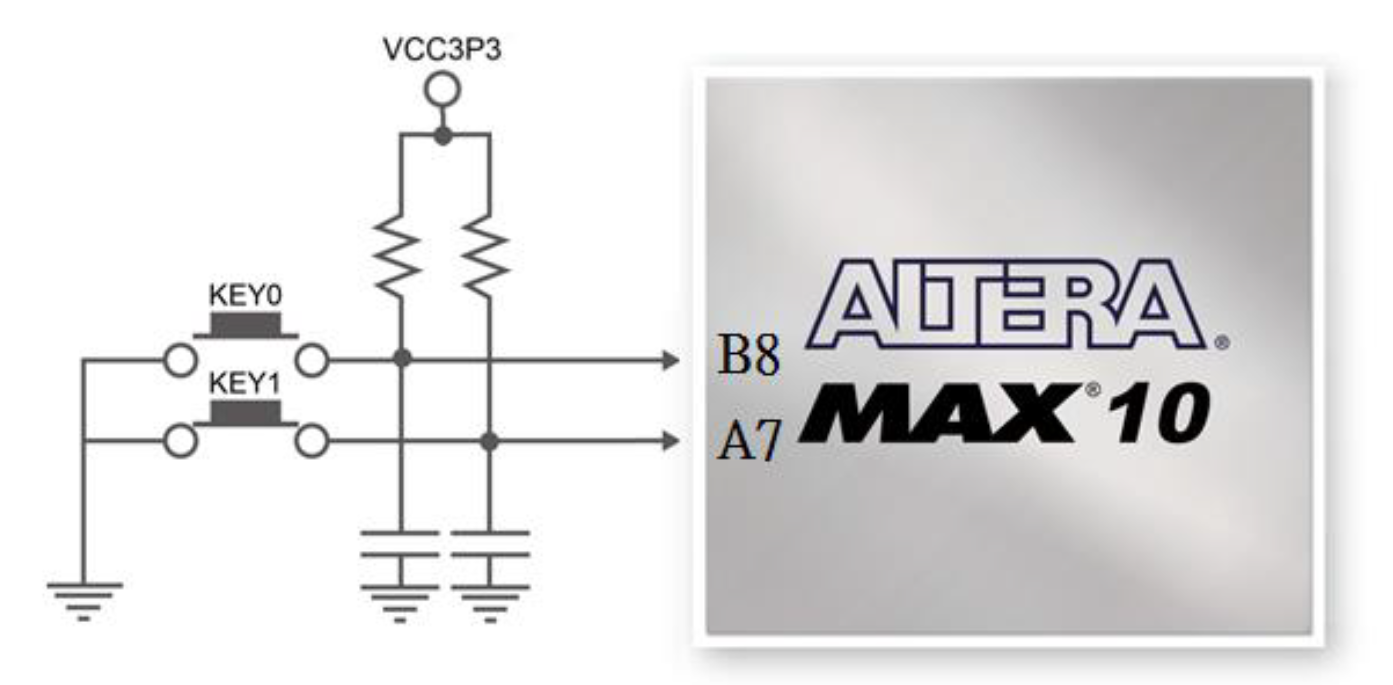
\includegraphics[width=0.8\linewidth]{images/controller/buttons.png}
    \caption{Connections between the push-button and MAX 10 FPGA.}
    \label{fig:push_buttons}
\end{figure}

According to the MAX 10 FPGA datasheet, these buttons are \textit{active-low}, meaning that a pressed button corresponds to a logic low signal (\texttt{0}), while an unpressed button corresponds to a logic high (\texttt{1}). 

\subsection{Asynchronous Reset with Synchronous Release}

The general reset is triggered when the user presses the button \texttt{KEY[0]}, which is connected to pin B8. This signal is processed using the \textbf{asynchronous reset with synchronous release} technique. This approach allows the controller to be reset asynchronously, ensuring an immediate response to the reset request. However, the release of the reset signal is synchronized with the clock, preventing potential metastability issues.

Without synchronous release, if the reset signal were deasserted exactly at the rising edge of the clock, it could lead to unpredictable behavior due to metastability. By synchronizing the reset deassertion with the clock, the system ensures a stable transition back to normal operation. Since the button is active-low, the controller is internally reset with a \texttt{$\mathtt{\sim}$ reset} signal. The architecture implementing this mechanism is illustrated in Fig.~\ref{fig:reset_architecture}.

\begin{figure}[!h]
    \centering
    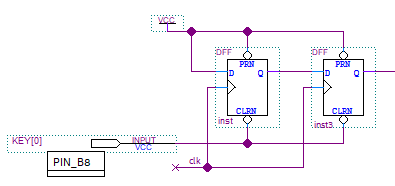
\includegraphics[width=0.8\linewidth]{images/controller/reset_circuit.png}
    \caption{Asynchronous Reset with Synchronous Release architecture.}
    \label{fig:reset_architecture}
\end{figure}

In this case, a debouncer circuit is not used because maintaining the asynchronous nature of the general reset is crucial. If the reset button is pressed multiple times, the resulting bouncing effect lasts only a few milliseconds, as indicated in the datasheet. This duration is significantly shorter than the minimum reset time required by the system, which is at least 120 ms (particularly for the LCD, as will be discussed in Section~\ref{sec:lt24_lcd_driver}). Consequently, multiple reset activations would not cause errors in the system.

\subsection{Rising Edge Detector} 

For the other push button, \texttt{KEY[1]}, which is connected to pin A7, a different approach is used. In this case, an asynchronous signal is not required; instead, the signal must be properly synchronized. More importantly, it must ensure that the transition allowing the state machine to proceed occurs only for a single clock cycle. To achieve this, a \textbf{debouncer} followed by a \textbf{rising edge detector} is implemented. As described for the reset button, the button is active low, so a NOT gate is implemented here before the other two mentioned blocks. Figure \ref{fig:button_circuit} shows the button circuit used.

\begin{figure}[!h]
    \centering
    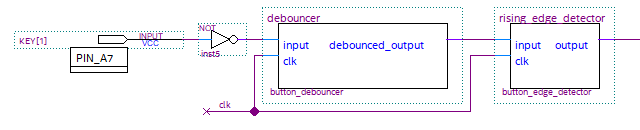
\includegraphics[width=0.8\linewidth]{images/controller/button_circuit.png}
    \caption{Button circuit.}
    \label{fig:button_circuit}
\end{figure}

The debouncer (shown in Fig.~\ref{fig:debounce_circuit}) is an optimized synchronizer specifically designed to eliminate signal bouncing. This is accomplished by down-sampling the input signal from the button using an enable-based technique. The same 50 MHz clock used for the entire system is utilized, but the enable signal allows the debouncer to sample at a reduced rate of \(50\text{ MHz}/2^{20} \simeq 50\text{Hz}\). This corresponds to a sampling period of 20 ms, which is approximately a decade away from the bouncing phenomenon, which typically ends within a few milliseconds.

\begin{figure}[!h]
    \centering
    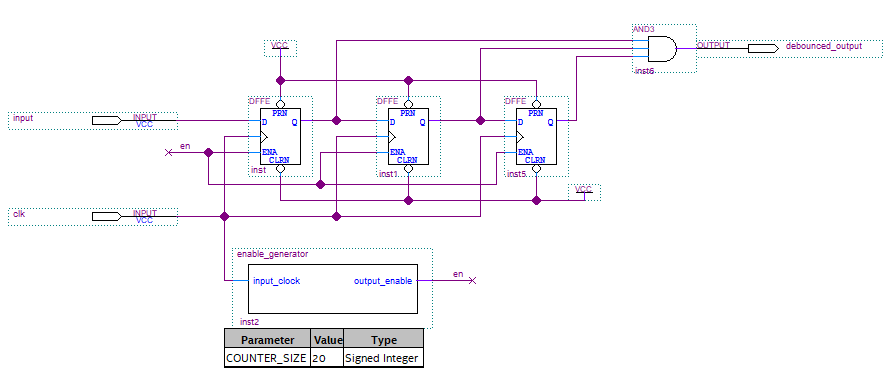
\includegraphics[width=0.8\linewidth]{images/controller/debounce_circuit.png}
    \caption{Debounce circuit.}
    \label{fig:debounce_circuit}
\end{figure}

Following the debouncer, a rising edge detector is implemented. Since the debounced signal remains high for the entire duration that the enable signal is active, a direct transition would not achieve the desired behavior. Instead, a rising edge detector, clocked at 50 MHz (illustrated in Fig.~\ref{fig:rising_edge_detector}), ensures that only a single clock cycle pulse is generated upon detecting a rising edge in the debounced signal. This guarantees that the button press is registered only once per press event, preventing unintended multiple transitions.

\begin{figure}[!h]
    \centering
    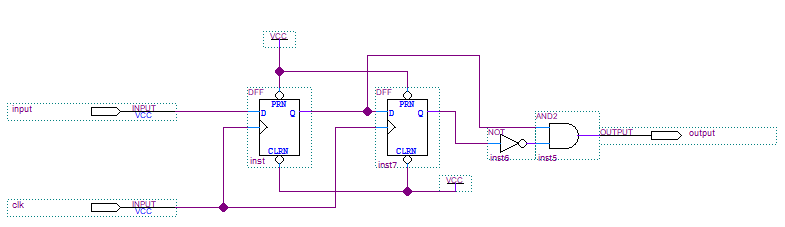
\includegraphics[width=0.8\linewidth]{images/controller/rising_edge_detector_circuit.png}
    \caption{Rising Edge Detector.}
    \label{fig:rising_edge_detector}
\end{figure}

\section{Seven-segment Display Driver}
\label{sec:seven_segment_driver}

The last section of this chapter is dedicated to the final output of the entire system, which is a seven-segment display used to represent the digit. Figure \ref{fig:seven_segments} shows the connection of the seven segments, where the LEDs of the segments are connected in a common-anode configuration to pins on the MAX 10 FPGA. Each segment can be turned on or off by applying a low logic level or high logic level from the FPGA, respectively. 

Each segment in the display is indexed from 0 to 6, along with the decimal point (dp). In this project, the second display (HEX1[0] to HEX1[7]) is used due to some issues with the first decimal point on the board. The decimal point is the default state, indicating to the user that the system is in all states except the \texttt{digit out} state.

\begin{figure}[!h]
    \centering
    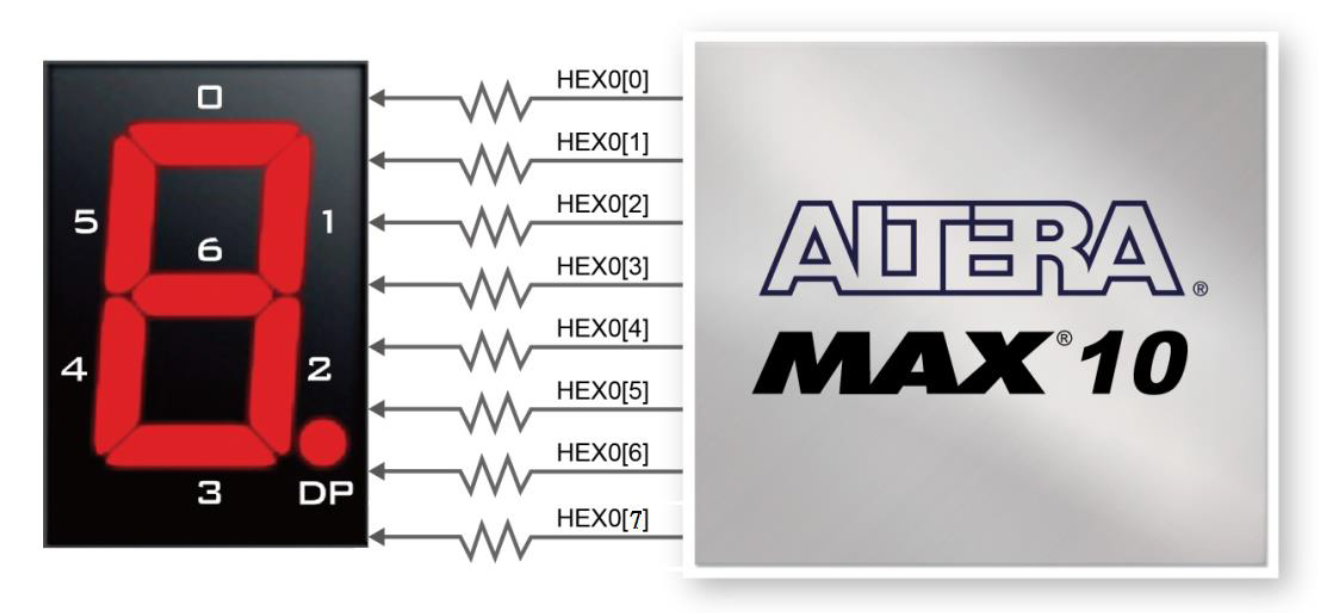
\includegraphics[width=0.8\linewidth]{images/controller/seven_segm.png}
    \caption{Connections between the 7-segment display HEX0 and the MAX 10 FPGA.}
    \label{fig:seven_segments}
\end{figure}

\chapter{Neural Network Design}

This chapter is organized as follows: Section~\ref{sec:intro} describes the possible neural networks present in the state of the art and provides a general description of the functioning of a neural network. Section~\ref{sec:neural_network_architecture} describes the architecture used in this work. Section~\ref{sec:training} details the process of training the data and quantizing the parameters of the neural network. Section~\ref{sec:digital_twin} presents the digital twin created to verify the correctness of the Verilog implementation. The following sections are dedicated to the Verilog modules.

\section{Definition}
\label{sec:intro}
In this project, the focus is on implementing a fully connected Multi-Layer Perceptron (MLP) neural network. While there are various types of neural networks, such as Convolutional Neural Networks (CNNs) and Recurrent Neural Networks (RNNs), which are more sophisticated and specialized for different tasks, this work aims to verify the feasibility of using artificial intelligence at the edge. Specifically, the objective is to implement neural networks on edge devices, in this case, on an FPGA, to evaluate their performance and practical applicability.

A neural network consists of multiple layers of interconnected nodes, commonly referred to as neurons. These neurons are loosely modeled after biological neurons in the human brain. Neural networks are typically composed of an input layer, one or more hidden layers, and an output layer. Each artificial neuron is connected to others and is associated with a weight and a threshold. When the weighted sum of inputs exceeds the threshold, the neuron activates and passes the data to the next layer. Otherwise, the information is not transmitted further.

The MLP used in this project follows this fundamental structure. It is a fully connected feedforward neural network where each neuron in a layer is connected to every neuron in the subsequent layer. The primary function of this network is to process input data through weighted connections, apply activation functions, and generate an output based on learned parameters. This simple yet powerful architecture makes MLPs suitable for a range of classification and regression tasks, particularly when deployed on resource-constrained environments like FPGAs.

Figure~\ref{fig:NN_example} shows the schematic example of a neural network.

\begin{figure}[!ht]
\centering
\resizebox{0.8\textwidth}{!}{% Reduce size of everything
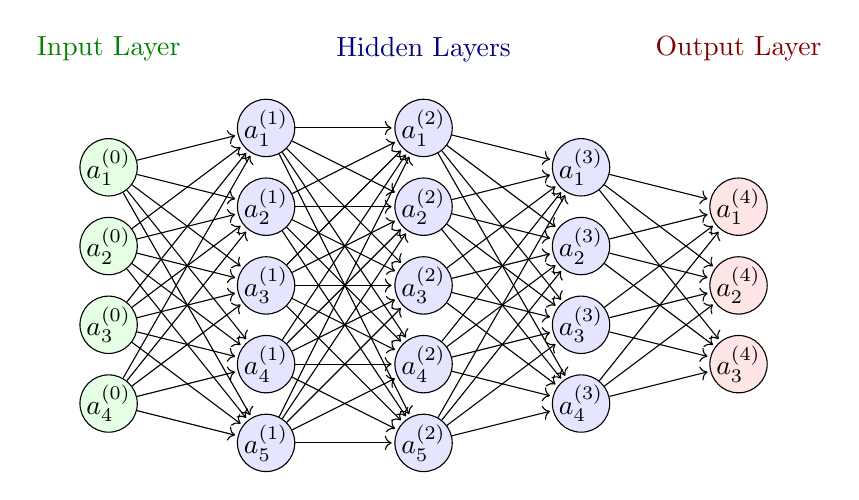
\begin{tikzpicture}[shorten >=1pt, node distance=1.5cm, on grid, auto]

    % Labels for entire layers
    \node[text=green!50!black] at (0,0) {Input Layer};
    \node[text=blue!50!black] at (4,0) {Hidden Layers};
    \node[text=red!50!black] at (8,0) {Output Layer};

    \node[circle, draw, fill=green!10, minimum size=6mm, inner sep=0pt] (I1) at (0,-1.5) {$a^{(0)}_{1}$};
    \node[circle, draw, fill=green!10, minimum size=6mm, inner sep=0pt] (I2) at (0,-2.5) {$a^{(0)}_{2}$};
    \node[circle, draw, fill=green!10, minimum size=6mm, inner sep=0pt] (I3) at (0,-3.5) {$a^{(0)}_{3}$};
    \node[circle, draw, fill=green!10, minimum size=6mm, inner sep=0pt] (I4) at (0,-4.5) {$a^{(0)}_{4}$};

    \node[circle, draw, fill=blue!10, minimum size=6mm, inner sep=0pt] (H11) at (2,-1) {$a^{(1)}_{1}$};
    \node[circle, draw, fill=blue!10, minimum size=6mm, inner sep=0pt] (H12) at (2,-2) {$a^{(1)}_{2}$};
    \node[circle, draw, fill=blue!10, minimum size=6mm, inner sep=0pt] (H13) at (2,-3) {$a^{(1)}_{3}$};
    \node[circle, draw, fill=blue!10, minimum size=6mm, inner sep=0pt] (H14) at (2,-4) {$a^{(1)}_{4}$};
    \node[circle, draw, fill=blue!10, minimum size=6mm, inner sep=0pt] (H15) at (2,-5) {$a^{(1)}_{5}$};

    \node[circle, draw, fill=blue!10, minimum size=6mm, inner sep=0pt] (H21) at (4,-1) {$a^{(2)}_{1}$};
    \node[circle, draw, fill=blue!10, minimum size=6mm, inner sep=0pt] (H22) at (4,-2) {$a^{(2)}_{2}$};
    \node[circle, draw, fill=blue!10, minimum size=6mm, inner sep=0pt] (H23) at (4,-3) {$a^{(2)}_{3}$};
    \node[circle, draw, fill=blue!10, minimum size=6mm, inner sep=0pt] (H24) at (4,-4) {$a^{(2)}_{4}$};
    \node[circle, draw, fill=blue!10, minimum size=6mm, inner sep=0pt] (H25) at (4,-5) {$a^{(2)}_{5}$};

    \node[circle, draw, fill=blue!10, minimum size=6mm, inner sep=0pt] (H31) at (6,-1.5) {$a^{(3)}_{1}$};
    \node[circle, draw, fill=blue!10, minimum size=6mm, inner sep=0pt] (H32) at (6,-2.5) {$a^{(3)}_{2}$};
    \node[circle, draw, fill=blue!10, minimum size=6mm, inner sep=0pt] (H33) at (6,-3.5) {$a^{(3)}_{3}$};
    \node[circle, draw, fill=blue!10, minimum size=6mm, inner sep=0pt] (H34) at (6,-4.5) {$a^{(3)}_{4}$};
    
    \node[circle, draw, fill=red!10, minimum size=6mm, inner sep=0pt] (O1) at (8,-2) {$a^{(4)}_{1}$};
    \node[circle, draw, fill=red!10, minimum size=6mm, inner sep=0pt] (O2) at (8,-3) {$a^{(4)}_{2}$};
    \node[circle, draw, fill=red!10, minimum size=6mm, inner sep=0pt] (O3) at (8,-4) {$a^{(4)}_{3}$};

    % Draw connections
    \foreach \i in {1,...,4} 
        \foreach \j in {1,...,5} 
            \draw[->] (I\i) -- (H1\j);
    \foreach \i in {1,...,5} 
        \foreach \j in {1,...,5} 
            \draw[->] (H1\i) -- (H2\j);
    \foreach \i in {1,...,5} 
        \foreach \j in {1,...,4} 
            \draw[->] (H2\i) -- (H3\j);
    \foreach \i in {1,...,4} 
        \foreach \j in {1,...,3} 
            \draw[->] (H3\i) -- (O\j);
    
\end{tikzpicture}
}
\caption{Layers of a Neural Network}
\label{fig:NN_example}
\end{figure}

\section{Neural Network Architecture}
\label{sec:neural_network_architecture}

The aim of this work is to develop a neural network capable of recognizing a handwritten digit (ranging from 0 to 9) provided through a touchscreen interface, as described in Chapter~\ref{chap:graphic_interface_design}. The Multi-Layer Perceptron (MLP) used in this work is structured as follows:

\begin{itemize}
    \item \textbf{Input Layer:} Consists of \textbf{196 pixels} in \textbf{8-bit precision}, obtained through an average pooling module, as described in Section~\ref{sec:average_pooling}.
    \item \textbf{Hidden Layer:} Composed of \textbf{32 fully connected neurons}, each producing an output in \textbf{24-bit precision}.
    \item \textbf{Output Layer:} Consists of \textbf{10 fully connected neurons}, where:
    \begin{itemize}
        \item The input to each neuron is in \textbf{24-bit precision}.
        \item The output of each neuron is also in \textbf{40-bit precision}.
    \end{itemize}
    \item \textbf{Predict Digit Module:} Selects the maximum value from the output layer to determine the predicted digit.
\end{itemize}

The neural network operates with the following precision settings:
\begin{itemize}
    \item \textbf{Weights and Biases:} Fixed at \textbf{8-bit precision}.
    \item \textbf{Input Layer:} Pixel values represented in \textbf{8-bit precision}.
    \item \textbf{Hidden Layer:} Inputs in \textbf{8-bit precision}, outputs in \textbf{24-bit precision}.
    \item \textbf{Output Layer:} Inputs in \textbf{24-bit precision}, outputs in \textbf{40-bit precision}.
\end{itemize}

It is important to note that the primary externally chosen parameter is the precision of weights and biases, which is set to 8-bit. The precision of internal signals is then adjusted accordingly to maintain full resolution throughout computations, preventing truncation errors that could lead to misinterpretations of the inputs. Consequently, different layers operate with different output resolutions to preserve computational accuracy.


Figure~\ref{fig:MLP} illustrates this structure.


\begin{figure}[!ht]
\centering
\resizebox{1\textwidth}{!}{% Reduce size of everything
\begin{tikzpicture}
\tikzstyle{every node}=[font=\small]

    % Labels for entire layers
    \node at (0,-6) {\normalsize Input Layer};
    \node at (4,-5.25) {\normalsize Hidden Layer};
    \node at (8,-5) {\normalsize Output Layer};

    % Define input layer nodes
    \node[circle, draw, fill=green!10, minimum size=6mm, inner sep=0pt] (I1) at (0,0) {$0$};
    \node[circle, draw, fill=green!10, minimum size=6mm, inner sep=0pt] (I2) at (0,-0.75) {$1$};
    \node[circle, draw, fill=green!10, minimum size=6mm, inner sep=0pt] (I3) at (0,-1.5) {$2$};
    \node[circle, draw, fill=green!10, minimum size=6mm, inner sep=0pt] (I4) at (0,-2.25) {$3$};
    \node[circle, draw, fill=green!10, minimum size=6mm, inner sep=0pt] (I5) at (0,-3) {$4$};
    \node at (0,-3.75) {\vdots};  % Ellipsis for hidden neurons
    \node[circle, draw, fill=green!10, minimum size=6mm, inner sep=0pt] (I195) at (0,-4.5) {$194$};
    \node[circle, draw, fill=green!10, minimum size=6mm, inner sep=0pt] (I196) at (0,-5.25) {$195$};

    % Define hidden layer nodes
    \node[circle, draw, fill=blue!10, minimum size=6mm, inner sep=0pt] (H1) at (4,-0.75) {$0$};
    \node[circle, draw, fill=blue!10, minimum size=6mm, inner sep=0pt] (H2) at (4,-1.50) {$1$};
    \node[circle, draw, fill=blue!10, minimum size=6mm, inner sep=0pt] (H3) at (4,-2.25) {$2$}
    \node at (4,-3) {\vdots};  % Ellipsis for hidden neurons
    \node[circle, draw, fill=blue!10, minimum size=6mm, inner sep=0pt] (H31) at (4,-3.75) {$30$};
    \node[circle, draw, fill=blue!10, minimum size=6mm, inner sep=0pt] (H32) at (4,-4.5) {$31$};

    % Define output layer nodes
    \node[circle, draw, fill=red!10, minimum size=6mm, inner sep=0pt] (O1) at (8,-1.25) {$0$};
    \node[circle, draw, fill=red!10, minimum size=6mm, inner sep=0pt] (O2) at (8,-2) {$1$};
    \node at (8,-2.75) {\vdots};  % Ellipsis for hidden neurons
    \node[circle, draw, fill=red!10, minimum size=6mm, inner sep=0pt] (O9) at (8,-3.50) {$8$};
    \node[circle, draw, fill=red!10, minimum size=6mm, inner sep=0pt] (O10) at (8,-4.25) {$9$};

    \node[rectangle, draw, fill=yellow!10, minimum size=6mm, inner sep=0pt] (pd) at (12,-2.75) {\normalsize Predict Digit};

    \node (out) at (16,-2.75) {\normalsize Digit Out};

    % Draw connections from input layer to hidden layer
    \draw[->] (I1) -- (H1);
    \draw[->] (I1) -- (H2);
    \draw[->] (I1) -- (H3);
    \draw[->] (I1) -- (H31);
    \draw[->] (I1) -- (H32);
    \draw[->] (I2) -- (H1);
    \draw[->] (I2) -- (H2);
    \draw[->] (I2) -- (H3);
    \draw[->] (I2) -- (H31);
    \draw[->] (I2) -- (H32);
    \draw[->] (I3) -- (H1);
    \draw[->] (I3) -- (H2);
    \draw[->] (I3) -- (H3);
    \draw[->] (I3) -- (H31);
    \draw[->] (I3) -- (H32);
    \draw[->] (I4) -- (H1);
    \draw[->] (I4) -- (H2);
    \draw[->] (I4) -- (H3);
    \draw[->] (I4) -- (H31);
    \draw[->] (I4) -- (H32);
    \draw[->] (I5) -- (H1);
    \draw[->] (I5) -- (H2);
    \draw[->] (I5) -- (H3);
    \draw[->] (I5) -- (H31);
    \draw[->] (I5) -- (H32);
    \draw[->] (I195) -- (H1);
    \draw[->] (I195) -- (H2);
    \draw[->] (I195) -- (H3);
    \draw[->] (I195) -- (H31);
    \draw[->] (I195) -- (H32);
    \draw[->] (I196) -- (H1);
    \draw[->] (I196) -- (H2);
    \draw[->] (I196) -- (H3);
    \draw[->] (I196) -- (H31);
    \draw[->] (I196) -- (H32);

    % Draw connections from hidden layer to output layer
    \draw[->] (H1) -- (O1);
    \draw[->] (H1) -- (O2);
    \draw[->] (H1) -- (O9);
    \draw[->] (H1) -- (O10);
    \draw[->] (H2) -- (O1);
    \draw[->] (H2) -- (O2);
    \draw[->] (H2) -- (O9);
    \draw[->] (H2) -- (O10);
    \draw[->] (H3) -- (O1);
    \draw[->] (H3) -- (O2);
    \draw[->] (H3) -- (O9);
    \draw[->] (H3) -- (O10);
    \draw[->] (H31) -- (O1);
    \draw[->] (H31) -- (O2);
    \draw[->] (H31) -- (O9);
    \draw[->] (H31) -- (O10);
    \draw[->] (H32) -- (O1);
    \draw[->] (H32) -- (O2);
    \draw[->] (H32) -- (O9);
    \draw[->] (H32) -- (O10);

    %predict digit
    \draw[->] (O1) -- (pd);
    \draw[->] (O2) -- (pd);
    \draw[->] (O9) -- (pd);
    \draw[->] (O10) -- (pd);

    \draw[->] (pd) -- (out);

\end{tikzpicture}
}
\caption{Structure of the MLP used in this work}
\label{fig:MLP}
\end{figure}

Each node of the hidden and output layers consists of a neuron and an activation layer. The first calculates the sum of the inputs weighted with each weight plus a bias, while the second is an activation function that inhibits low inputs and accentuates high inputs. In this way, activation functions reflect the behavior of neurons, where neurons require an input above a certain threshold to activate. For this work, a ReLU (Rectified Linear Unit) activation function is used, which is simply defined as \( y = \max(0, a) \). Figure \ref{fig:node} shows a functioning node.

\begin{figure}[!ht]
\centering
\resizebox{0.8\textwidth}{!}{% Reduce size of everything
\begin{tikzpicture}
\tikzstyle{every node}=[font=\small]

    \node (I1) at (0,0) {$x_0$};
    \node (I2) at (0,-0.75) {$x_1$};
    \node (I3) at (0,-1.5) {$x_2$};
    \node (I4) at (0,-2.25) {$x_3$};
    \node (I5) at (0,-3) {$x_4$};

    \node[circle, draw, fill=green!10, minimum size=6mm, inner sep=0pt] (neu) at (2,-1.50) {$\sum$};

    \node (bias) at (2,0) {$b$}

    \node[circle, draw, fill=red!10, minimum size=6mm, inner sep=0pt] (relu) at (4,-1.50) {$ReLu$};

    \node (out) at (6,-1.50) {$y$};

    \draw[->] (I1) -- (neu) node[midway, above] {$w_0$};
    \draw[->] (I2) -- (neu);
    \draw[->] (I3) -- (neu);
    \draw[->] (I4) -- (neu);
    \draw[->] (I5) -- (neu) node[midway, below] {$w_4$};

    \draw[->] (neu) -- (relu) node[midway, above] {$a$};

    \draw[->] (bias) -- (neu);

    \draw[->] (relu) -- (out);

\end{tikzpicture}
}
\caption{Structure of a node}
\label{fig:node}
\end{figure}

\section{Training}
\label{sec:training}

To obtain the appropriate weights and biases for implementing the neural network, it was necessary to train the network offline using a Jupyter Notebook script with Keras library. The case study in this work is a classical one in the neural network field and is well known. Therefore, we used the MNIST dataset, provided by the Modified National Institute of Standards and Technology (MNIST), as both the training and testing batches for the Python script. The dataset consists of 28x28 pixel images, corresponding to 784 input neurons. The first step in processing the data is to apply average pooling, reducing the dimensions to a 14x14 matrix. After this, the neural network described previously is applied.

Without delving into the details of neural networks, the training process involves not only the feedforward procedure but also backpropagation. This process allows the network to adjust the weights and biases to find the optimal values. The Python script also provides the accuracy of our model. Since the model was initially developed using floating-point numbers, it was necessary to quantize it to obtain a final batch of weights and biases in 8-bit format. This quantization is crucial for FPGA implementation, as it helps reduce the usage of the limited resources available on the FPGA.

The MNIST dataset consists of 70,000 handwritten images. For the purpose of this work, the dataset is split into 60,000 training images and 10,000 test images. Listing \ref{list:NN_python_keras} shows the construction of the neural network by stacking all the required layers, after downloading the data and converting the pixel values to 32-bit floating-point format.

\begin{lstlisting}[
language=Python,
style=python,
caption=Neural Network Construct in Python used for training the model,
label= list:NN_python_keras]
# Importing Keras model and layers
from keras.models import Sequential
from keras.layers import Dense, Flatten, AveragePooling2D

# Construct the NN by stacking all required layers
model_s_nn = Sequential() # Sequential: the layers will be connected to one another
model_s_nn.add(AveragePooling2D(pool_size=(2, 2), input_shape=(28, 28, 1)))
model_s_nn.add(Flatten()) # Flattening the 2D arrays for fully connected layers
model_s_nn.add(Dense(32, activation=tf.nn.relu))
model_s_nn.add(Dense(10,activation=tf.nn.softmax))
\end{lstlisting}

After constructing the neural network, the model was trained using the training dataset. For each image \( x_{\text{train}}(i) \), the model attempts to predict the associated digit \( y_{\text{train}}(i) \). It gradually adjusts the weights and biases of the dense layers during training, which was performed over 10 epochs. The final result is a model with an accuracy of approximately 97\%, which is quite good. To ensure that the model performs well on new data, its accuracy was then evaluated using the test dataset, by performing only the forward pass, resulting in an accuracy of 96\%. Figure \ref{fig:accuracy_over_epoch} shows the accuracy change over the epochs.

\begin{figure*}[!ht]
     \centering
     \subfloat[]{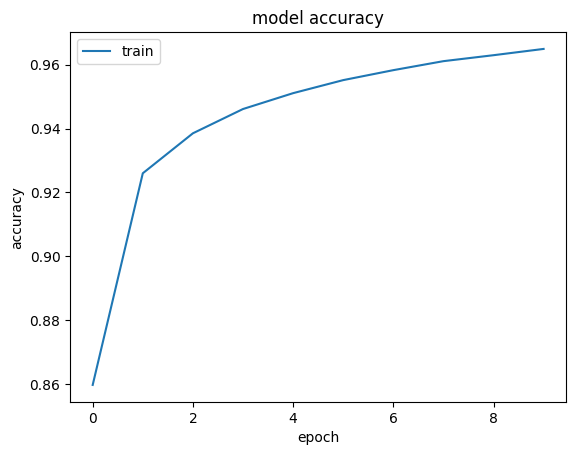
\includegraphics[width=0.5\linewidth]{images/neural_network/model_accuracy.png}%
    \label{fig:model_acc}}
    \hfil
    \subfloat[]{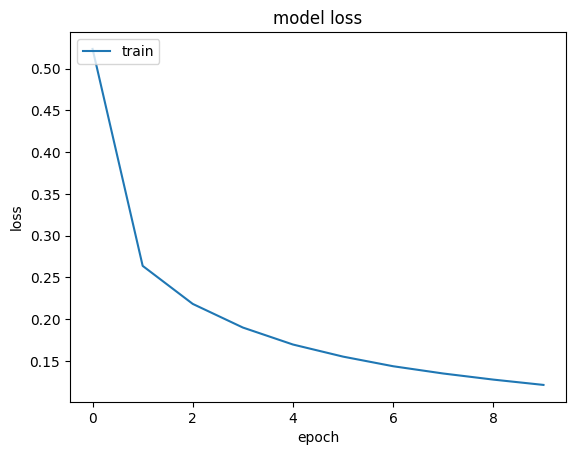
\includegraphics[width=0.5\linewidth]{images/neural_network/model_loss.png}%
    \label{fig:model_loss}}

     \caption{History of the model accuracy (a) and losses (b) over the training epochs.}
    \label{fig:accuracy_over_epoch}
\end{figure*}

Once the training was completed, it was necessary to quantize the weights and biases to achieve 8-bit precision. The function used to accomplish this goal is shown in \ref{list:quantize}.

\begin{lstlisting}[
language=Python,
style=python,
caption=Quantize Function,
label= list:quantize]
# Returns a quantized array
# Arguments:
# use_scale       If non-zero it will use this instead of auto-computing the scaling factor.
# Returns:
# out             The quantized data
# out_int         The quantized data, but scaled to an int value in the range +/- (2**n_bit-1)-1
# scale           The scaling factor used between out and out_int

def quantize_nbit(data, n_bit, use_scale=0, verbose=0):
    max_bit_val = (2**(n_bit-1))-1
    max_val     = np.max(np.abs(data))
    if use_scale > 0:
        scale = use_scale
    else :
        scale   = max_bit_val / max_val
    if verbose:
        print('Quantizing to +/- {}, scaling by {}'.format(max_bit_val, scale))

    out_int = np.around(data * scale)
    out = out_int /  scale

    return out, out_int, scale
\end{lstlisting}

As can be seen, the quantization is performed by taking the maximum value of the input vector and setting it to the maximum value for 8-bit precision, if \texttt{use\_scale} is set to 0. Otherwise, the value passed as a parameter is used. This approach is used because the scale factor is determined based on the weights vector of each layer, while the bias layer is quantized using the same scale factor as its corresponding weights. In this way, the quantization is achieved, and the weights and biases of each layer are then converted to Verilog format (8'bxxxxxxxx) using a script to accelerate the process.

\section{Digital Twin}
\label{sec:digital_twin}

In order to test the correctness of the Verilog implementation, it is useful to create a Python implementation of the quantized neural network as a digital twin. \ref{list:digital_twin} provides the code for this implementation.

\begin{lstlisting}[
language=Python,
style=python,
caption=Digital Twin,
label= list:digital_twin]
# **Average Pooling Function**
def average_pooling(matrix, pool_size=2):
    """
    Apply average pooling on input matrix, with given pool size
    """
    new_h, new_w = matrix.shape[0] // pool_size, matrix.shape[1] // pool_size
    pooled_matrix = np.zeros((new_h, new_w), dtype=np.int8)

    for i in range(new_h):
        for j in range(new_w):
            idx_x, idx_y = i * pool_size, j * pool_size
            block = matrix[idx_x:idx_x + pool_size, idx_y:idx_y + pool_size]
            pooled_matrix[i, j] = np.sum(block) // pool_size**2  # Integer division for mean

    return pooled_matrix

# **Forward Pass for a Single Layer**
def layer_forward(inputs, weights, biases, verbose=False):
    """
    Perform a forward pass through a single layer:
    - Multiply-Accumulate (MAC) operation.
    - Apply ReLU.
    """
    # Compute MAC
    mac = np.dot(inputs.astype(np.int32), weights.T.astype(np.int32)) + biases.astype(np.int32)
    if verbose:
      print(f"Dense out:\n{mac}")

    # Apply ReLU
    return np.maximum(mac, 0)

# **Decision Function**
def decision(outputs):
    """
    Return the index of the maximum output (final prediction).
    """
    return np.argmax(outputs)

# Step 1: Average Pooling (28x28 -> 14x14)
pooled = average_pooling(input_image)

# Step 2: Flatten to 196 elements
input_feature = pooled.flatten().astype(np.int8)

# **MLP Forward Pass**
# Hidden Layer
layer1_output = layer_forward(input_feature, weights_HL, biases_HL, verbose=True)

# Output Layer
layer2_output = layer_forward(layer1_output, weights_OL, biases_OL, verbose=True)

# Decision Block
predicted_digit = decision(layer2_output)
\end{lstlisting}

It is important to note that in the provided code, the weights and biases vectors are omitted for clarity. This code is used to test the accuracy of the quantized model, achieving an accuracy of 95.75\%, demonstrating that the quantization process practically does not degrade the model's performance. Finally, a script is written to generate the same input as in the final hardware implementation, which is useful for debugging the Verilog code and verifying the correctness of the work done.

\section{Verilog Implementation}

In this section, the Verilog implementation of each module is presented.


\subsection{Forward Logic Finite State Machine}

The \textbf{Forward Logic FSM} sub-system performs the following tasks:

\begin{itemize}
    \item It implements a \textbf{Finite State Machine (FSM)} to control the flow through different stages.
    \item It receives the \textbf{preprocessed pixel data} from the input layer and initiates the feedforward computation.
    \item It manages the execution flow of a \textbf{Multi-Layer Perceptron (MLP)} network, ensuring the correct sequencing of operations for digit prediction, activating the hidden and output layers to generate the activation values..
    \item It triggers the \textbf{digit prediction module}, which processes the activations from the output layer and determines the predicted digit.
    \item It provides a \textbf{done signal} to indicate when the entire computation process is completed.
\end{itemize}

The Quartus block of this sub-system is shown in Fig. \ref{fig:FW_logic_FSM}.

\begin{figure}[!h]
    \centering
    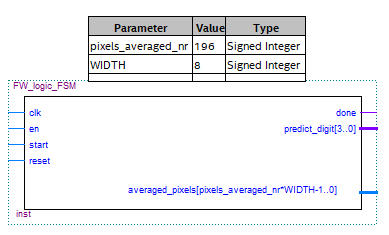
\includegraphics[width=0.6\linewidth]{images/neural_network/nn_quartus_block.png}
    \caption{Quartus block of Forward Logic FSM sub-system.}
    \label{fig:FW_logic_FSM}
\end{figure}

\begin{lstlisting}[
language=Verilog,
style=verilog,
caption=FW\_logic\_FSM declaration,
label= list:FW_logic_FSM_declaration]
module FW_logic_FSM #(
    parameter pixels_averaged_nr = 196, // Number of input pixels
    parameter WIDTH = 8
)( 
    input clk,
    input reset,
    input start,
    input [pixels_averaged_nr*WIDTH-1:0] averaged_pixels, // Flattened input pixel data
    input en,
    output [3:0] predict_digit, // Output predicted digit
    output reg done // Done signal indicating completion
);
\end{lstlisting}

Listing~\ref{list:FW_logic_FSM_declaration} shows the declaration of the parameters, inputs, and outputs of this module. As previously mentioned, the inputs consist of 196 pixels obtained from the average pooling module, which operates externally to this logic.  

The key parameter \texttt{WIDTH} defines the bit precision of weights and biases, set to 8-bit. The module outputs include the predicted digit and a \texttt{done} signal, which ensures that the control logic triggers the display of the result on the seven-segment display.

Figure \ref{fig:FW_logic_FSM} shows the flow diagram.

\begin{figure}[!ht]
\centering
\resizebox{1\linewidth}{!}{% Reduce size of everything
\begin{tikzpicture}[shorten >=1pt, node distance=2cm and 3cm, on grid, auto] 

   %\draw[help lines] (0,-5) grid (10,10);
   % Define the states with text wrapping
   \node[] (reset_in) at (-2,0) {};
   
   \node[state] (reset)   {RESET}; 
   \node[state] (idle) [right=of reset] {IDLE}; 
   \node[state] (mlp_start) [above right=of idle] {MLP START}; 
   \node[state] (mlp_wait) at (11, 2) {MLP WAIT};
   \node[state, text width=2cm, align=center] (predict_digit_start) at (16, 0) {PREDICT DIGIT START};
   \node[state, text width=2cm, align=center] (predict_digit_wait) at (11, -2) {PREDICT DIGIT WAIT};
   \node[state] (digit_out) at (6, -2) {DIGIT OUT};

   % Define transitions
   \path[->,every node/.style={font=\footnotesize}]
    (reset_in) edge node {reset} (reset)
    (reset) edge  node {} (idle)
    (idle) edge  node {start} (mlp_start)
          edge [loop below] node {!start} ()
    (mlp_start) edge node {} (mlp_wait)
    (mlp_wait) edge node {MLP\_done} (predict_digit_start)
          edge [loop above] node {!MLP\_done} ()
    (predict_digit_start) edge node {} (predict_digit_wait)
    (predict_digit_wait) edge node {predict\_digit\_done} (digit_out)
          edge [loop below] node {!predict\_digit\_done} ()
    (digit_out) edge node {} (idle);
    
\end{tikzpicture}
}
\caption{Forward Logic FSM: flux diagram}
\label{fig:FW_logic_FSM}
\end{figure}

The FSM operates as a Moore machine, where the state determines the output signals. The behavior of each state is described as follows:

\begin{itemize}
    \item \textbf{RESET:} All control signals are set to zero, ensuring the system is properly initialized.
    \item \textbf{IDLE:} The system remains in a waiting state until the start signal is received, with all control signals inactive.
    \item \textbf{MLP\_START:} The MLP computation begins by asserting the \texttt{MLP\_go} signal.
    \item \textbf{MLP\_WAIT:} The FSM waits for the MLP computation to complete, keeping all control signals deactivated.
    \item \textbf{PREDICT\_DIGIT\_START:} The digit prediction process is initiated by asserting the \texttt{predict\_digit\_go} signal.
    \item \textbf{PREDICT\_DIGIT\_WAIT:} The FSM waits for the completion of the digit prediction process, with control signals inactive.
    \item \textbf{DIGIT\_OUT:} The FSM signals completion by setting \texttt{done} to 1, indicating that the predicted digit is ready.
\end{itemize}


\subsection{MLP}

The \textbf{MLP (Multi-Layer Perceptron)} sub-system performs the following tasks:

\begin{itemize}
    \item It implements a simple \textbf{fully connected neural network structure} with a hidden layer and an output layer.
    \item It processes \textbf{input features}, which are the averaged pixels (flattened into a vector), using the \textbf{MLP computation}.
    \item The system starts the computation when the \texttt{MLP\_go} signal is activated.
    \item The \textbf{hidden layer} performs the transformation of input features into hidden activations. The number of neurons in the hidden layer is configurable, with 32 neurons in this case, and the output of the hidden layer is passed to the next stage for further processing.
    \item The \textbf{output layer} processes the activations from the hidden layer to produce the final output. The number of output neurons is 10, corresponding to the 10 possible digit predictions (0 to 9).
    \item The system waits for the completion of both the hidden layer and output layer computations using the \texttt{hidden\_done} and \texttt{MLP\_done} signals, respectively, ensuring the correct sequencing of operations.
    \item Once the output layer computation is complete, the \texttt{MLP\_done} signal is raised, indicating that the entire computation process is finished and the activations are ready.
\end{itemize}

The structure is split into two major sub-modules:

\begin{itemize}
    \item \textbf{Hidden layer:} This module performs the transformation of the input features through the hidden neurons. The number of hidden neurons is set to 32.
    \item \textbf{Output layer:} This module processes the hidden activations to produce the final predictions. The number of output neurons is set to 10 for digit classification.
\end{itemize}

The \textbf{MLP} module encapsulates the operations of these two layers and controls the flow of data between them using the internal control signals.

\begin{lstlisting}[
language=Verilog,
style=verilog,
caption=MLP declaration,
label= list:MLP_declaration]
module MLP #(
    //constants
    parameter averaged_pixels_nr = 196, // Number of input features
    parameter WIDTH = 8, // Bit width for input and weights
    parameter HL_neurons = 32, // Number of neurons in the hidden layer
    parameter OL_neurons = 10 // Number of neurons in the output layer
    )(
    input clk,
    input reset,
    input MLP_go,
    input [WIDTH*averaged_pixels_nr-1:0] averaged_pixels,
    output MLP_done,
    output [5*WIDTH*OL_neurons-1:0] output_activations
    );
\end{lstlisting}

Listing \ref{list:MLP_declaration} shows the declaration of the \textbf{MLP} module, where the number of neurons in the hidden layer is defined as 32, and the number of neurons in the output layer is defined as 10. This block is triggered by the \texttt{MLP\_go} signal (which directly triggers the hidden layer), and its output consists of two key signals: the \texttt{MLP\_done} signal, which indicates the completion of the MLP computation, and the output activations from the output layer.

Internally, this module simply instantiates the two layers—\textbf{hidden layer} and \textbf{output layer}—which are interconnected through internal signals. These internal signals include:

\begin{itemize}
    \item \texttt{hidden\_done}: A signal indicating that the hidden layer computation is complete.
    \item \texttt{hidden\_out}: The output from the hidden layer, which becomes the input to the output layer.
\end{itemize}

\subsection{Hidden and Output Layer}

Both the \textbf{Hidden Layer} and \textbf{Output Layer} modules are structurally identical, consisting of the instantiation of a fully connected dense layer followed by a ReLU activation layer. The input to the Hidden Layer comes from the preprocessed input features, while the Output Layer receives its input from the Hidden Layer's output activations.

These two modules define the weights and biases as \texttt{localparam} constants, which are stored as flattened vectors and passed to the dense layer. Listing \ref{list:hidden_layer_declaration} and \ref{list:output_layer_declaration} presents the declarations for both the Hidden and Output Layer modules. 

\begin{lstlisting}[
language=Verilog,
style=verilog,
caption=hidden\_layer declaration,
label= list:hidden_layer_declaration]
module hidden_layer #(
    parameter averaged_pixels_nr = 196, // Input pixels number
    parameter WIDTH = 8,
    parameter HL_neurons = 32 // Neuron number for the hidden layer
	)(
    input clk,
    input hidden_go,
    input reset,
    input signed [WIDTH*averaged_pixels_nr-1:0] hidden_in,
    output signed [3*WIDTH*HL_neurons-1:0] hidden_out,
    output hidden_done // Signals indicating completion of computation
    );
\end{lstlisting}

\begin{lstlisting}[
language=Verilog,
style=verilog,
caption=output\_layer declaration,
label= list:output_layer_declaration]
module output_layer #(
  parameter HL_neurons = 32, // Neurons number of the previous layer
  parameter WIDTH = 8,
  parameter OL_neurons = 10 // Neurons number of the output layer
	)(
  input clk,
  input output_go,
  input reset,
  input signed [3*WIDTH*HL_neurons-1:0] output_in, // Input from the hidden layer
  output signed [5*WIDTH*OL_neurons-1:0] output_out, // Output activations after ReLU
  output output_done // Signal indicating completion of computation
  );
\end{lstlisting}

In the description of this module, after instantiating the weights and biases, the \textbf{Dense Layer} and \textbf{ReLU Activation Layer} instances are created. In accordance with Section \ref{sec:neural_network_architecture}, these layers operate with specific bit-width configurations optimized for different stages of computation.

\begin{itemize}
    \item The \textbf{Hidden Layer} dense computation (\texttt{hidden\_dense}) utilizes \textbf{8-bit precision} for both weights and biases (\texttt{WIDTH}). The input data is also in 8-bit precision (\texttt{WIDTH\_IN = WIDTH}), while the output expands to \textbf{24-bit precision} (\texttt{WIDTH\_OUT = 3*WIDTH}) to prevent truncation errors and preserve numerical accuracy for subsequent operations.
    \item The \textbf{Output Layer} follows a similar design, maintaining \textbf{8-bit precision} for weights and biases but processing \textbf{24-bit precision} inputs and generating \textbf{40-bit precision} outputs (\texttt{WIDTH\_OUT = 5*WIDTH}). This increased precision is necessary to accommodate the accumulated results from previous layers.
    \item The \textbf{ReLU Activation Layer} in both cases operates with the same bit-width for inputs and outputs as the dense layer it follows, ensuring consistent precision through the activation stage.
\end{itemize}

To coordinate the computational flow, dedicated control signals propagate through the layers. The \texttt{done} signal transitions from the dense layer to the ReLU activation layer and ultimately exits the module, signaling the completion of processing. This structured approach ensures efficient parallel computation and precise data representation across the network.  

\subsection{Dense Layer}

The \textbf{Dense Layer} module is a responsible for computing neuron activations by applying learned weights and biases to the input data. It consists of multiple neuron instances, each performing a weighted sum of its inputs followed by the addition of a bias term. Once all neurons complete their computations, the module generates a \texttt{done} signal to indicate the completion of the layer’s operation.  

This module is designed to handle different bit-width configurations to accommodate the varying input data precision across layers. The input features are distributed in parallel to all neurons, ensuring that each neuron receives the corresponding weight and bias values. The weighted sums are then computed, producing neuron activations that will be passed to subsequent processing stages, such as activation functions. This structure enables efficient parallel computation and streamlined data flow between layers.  

Since Verilog does not support passing matrices between modules, the weights are represented as a flattened vector. Consequently, the module slices the weight vector appropriately to provide each neuron with its corresponding set of weights. 

Listing \ref{list:dense_layer_declaration} presents the dense layer declaration.  

\begin{lstlisting}[
language=Verilog,
style=verilog,
caption=dense\_layer declaration,
label= list:dense_layer_declaration]
module dense_layer # (
    parameter NEURON_NB = 32, // Number of neurons in the dense layer
    parameter IN_SIZE = 196, // Number of input features per neuron
    parameter WIDTH = 8, // Bit width for weights and biases
    parameter WIDTH_IN = 8, // Bit width of the input data
    parameter WIDTH_OUT = 32 // Bit width of the output data
    )(
    input clk,
    input dense_go, // Start signal for computation
    input reset,
    input signed [WIDTH_IN*IN_SIZE-1:0] dense_in, // Flattened input data array
    input signed [WIDTH*NEURON_NB*IN_SIZE-1:0] weights,
    input signed [WIDTH*NEURON_NB-1:0] biases,
    output signed [WIDTH_OUT*NEURON_NB-1:0] dense_out, // Output activations
    output dense_done // Signal indicating completion of computation
    );     
\end{lstlisting}

\subsection{Neuron}

The \textbf{Neuron} module performs the following tasks:

\begin{itemize}
    \item It manages the flow of data and correctly provides inputs for the Multiply-Accumulate (MAC) module, which performs the actual weighted sum computation.
    \item It controls the sequencing of operations through a finite state machine (FSM), ensuring proper synchronization of data processing.
    \item It slices the flattened input data and weight vectors, ensuring each input feature is mapped to its corresponding weight before being sent to the MAC module.
    \item It monitors the computation progress using a counter (\textbf{index}) that tracks the number of processed inputs (\textbf{IN\_SIZE}). Once all inputs have been computed by the MAC module, the neuron adds the bias term to finalize the activation value.
    \item It generates a \texttt{done} signal to indicate when the neuron has completed processing all input features.
\end{itemize}

To better understand the functioning of this module, listing \ref{list:neuron_declaration} presents the neuron declaration.  

\begin{lstlisting}[
language=Verilog,
style=verilog,
caption=neuron declaration,
label= list:neuron_declaration]
module neuron #(
    parameter IN_SIZE = 196, // Number of input neurons
    parameter WIDTH = 8, // Bit width of input data and weights
    parameter WIDTH_IN = 8, // Bit width of the input data
    parameter WIDTH_OUT = 24 // Bit width of the output neuron value
)(
    input clk,                                     // Clock signal
    input reset,                                   // Reset signal
    input neuron_go,                               // Start signal to begin processing
    input [WIDTH_IN*IN_SIZE-1:0] in_data,          // Flattened input data
    input [WIDTH*IN_SIZE-1:0] weight,              // Flattened weights
    input signed [WIDTH-1:0] bias,                 // Bias input
    output signed [WIDTH_OUT-1:0] output_neuron,   // Output neuron value
    output neuron_done
);    
\end{lstlisting}

\begin{figure}[!ht]
\centering
\resizebox{1\linewidth}{!}{% Reduce size of everything
\begin{tikzpicture}[shorten >=1pt, node distance=2cm and 3cm, on grid, auto] 

   % Define the states with text wrapping
   \node[] (reset_in) [left=of reset] {};
   
   \node[state] (reset)   {RESET}; 
   \node[state] (idle) [right=of reset] {IDLE}; 
   \node[state] (mac) [above right=of idle] {MAC}; 
   \node[state] (output) [below right=of idle] {OUTPUT};

   % Define transitions
   \path[->]
    (reset_in) edge node {reset} (reset)
    (reset) edge  node {} (idle)
    (idle) edge  node {neuron\_go} (mac)
          edge [loop below] node {!neuron\_go} ()
    (mac) edge node {index==IN\_SIZE-1} (output)
          edge [loop above] node {index!=IN\_SIZE-1} ()
    (output) edge node {} (idle);
    
\end{tikzpicture}
}
\caption{Neuron: flux diagram}
\label{fig:neuron_FSM}
\end{figure}

Figure \ref{fig:neuron_FSM} shows the flow diagram. The finite state machine operates as follows:  

\begin{itemize}
    \item \textbf{RESET:}  
    \begin{itemize}
        \item All control signals for the counter and the signed multiply-and-accumulate (MAC) module are reset to their default values.  
        \item \texttt{mac\_aclr} is asserted to clear the MAC register, ensuring no residual values affect the computation.  
        \item \texttt{count\_en} is deactivated to prevent unintended increments.  
    \end{itemize}
    
    \item \textbf{IDLE:}  
    \begin{itemize}
        \item The system remains in an idle state, maintaining the same signal values as in the reset state, except for \texttt{mac\_aclr}, which is deasserted to allow normal operation.  
        \item It waits for the assertion of \texttt{neuron\_go}, which signals the start of computation.  
    \end{itemize}
    
    \item \textbf{MAC:}  
    \begin{itemize}
        \item The MAC operation begins, accumulating weighted sums over multiple clock cycles.  
        \item \texttt{mac\_clken} is asserted, enabling the MAC module to perform computations.  
        \item \texttt{count\_en} is activated, allowing the counter to increment and iterate through the input data.  
        \item \texttt{mac\_aclr} remains deasserted, ensuring accumulation continues without being reset.  
        \item The counter output (\texttt{index}) determines the appropriate portions of \texttt{in\_data} and \texttt{weight} for the MAC module.  
        \item \texttt{sload} is asserted at the start of the computation to initialize the MAC register with the first weighted input.  
    \end{itemize}
    
    \item \textbf{OUTPUT:}  
    \begin{itemize}
        \item When \texttt{index} reaches \texttt{IN\_SIZE-1}, the accumulation process is complete.  
        \item \texttt{mac\_clken} is deactivated to stop further computations.  
        \item \texttt{mac\_aclr} is asserted, clearing the \texttt{old\_result} register to prepare for a new input.  
        \item The final MAC result is stabilized and passed to the next processing stage (ReLU).  
        \item \texttt{done} is asserted, signaling the completion of neuron computation.  
    \end{itemize}
\end{itemize}

\subsection{Signed Multiply And Accumulate}  

For this module, a Quartus template is used, allowing the synthesizer to recognize the multiply-accumulate (MAC) structure and implement it using embedded multipliers instead of logic elements.  

It is important to highlight the control signals of this module:  

\begin{itemize}
    \item \textbf{\texttt{clken}:} Acts as the enable signal for the output flip-flop.  
    \item \textbf{\texttt{sload}:}  
    \begin{itemize}
        \item Used to reset the accumulated result when all neuron inputs have been processed.  
        \item Internally, a register \texttt{old\_result} is defined to store the previous result when \texttt{sload} is not asserted, allowing for continuous accumulation.  
    \end{itemize}
    \item \textbf{\texttt{aclr}:} A synchronous reset used to reset the register. When set to 1, it clears the stored data; when set to 0, it allows data to be updated as appropriate.  
\end{itemize}
 

This structure enables the implementation of a signed multiply-and-accumulate operation efficiently.

\subsection{ReLU Layer}  

The \textbf{ReLU Layer} module has a structure similar to the dense layer, but instead of instantiating neurons, it instantiates multiple ReLU activation modules. It processes the neuron outputs in parallel, ensuring that all negative values are set to zero while positive values remain unchanged.  

The main characteristics of this module are:  

\begin{itemize}
    \item It instantiates \texttt{NEURON\_NB} ReLU activation modules, each applied to the corresponding neuron output.
    \item It takes as input a flattened array \texttt{data\_in\_array} containing the neuron outputs from the dense layer.
    \item Each ReLU instance processes its respective input independently and outputs the activated value in the \texttt{data\_out\_array}.
    \item The module starts processing when the \texttt{relu\_go} signal is asserted.
    \item The \texttt{relu\_layer\_done} signal is asserted when all ReLU computations have been completed.
\end{itemize}  

Listing~\ref{list:relu_layer_declaration} presents the ReLU layer declaration.

\begin{lstlisting}[
language=Verilog,
style=verilog,
caption=relu\_layer declaration,
label= list:relu_layer_declaration]
module ReLU_layer #(
    parameter NEURON_NB = 10,  
    parameter WIDTH = 32
) (
    input clk,
    input reset,
    input relu_go,
    input [WIDTH*NEURON_NB-1:0] data_in_array, // Flattened 1D array for inputs
    output relu_layer_done,
    output [WIDTH*NEURON_NB-1:0] data_out_array // Flattened 1D array for outputs
);    
\end{lstlisting}

\subsection{ReLU}  

The \textbf{ReLU} (Rectified Linear Unit) module applies the activation function defined as:  
\[
f(x) = \max(0, x)
\]
where negative inputs are set to zero, and positive inputs remain unchanged.  

The main characteristics of this module are:  

\begin{itemize}
    \item It operates on a single input value \texttt{data\_in} and produces the corresponding activated output \texttt{data\_out}.
    \item The computation is performed in a \textbf{single clock cycle}.
    \item When the \texttt{relu\_go} signal is asserted, the module processes \texttt{data\_in} and updates \texttt{data\_out}.
    \item The \texttt{relu\_done} signal is asserted in the same clock cycle as \texttt{relu\_go}, indicating that the activation process has completed.
    \item The module resets \texttt{data\_out} to zero when the reset signal is active.
\end{itemize}  

This efficient design allows for seamless integration into the neural network pipeline.  
Listing~\ref{list:relu_declaration} presents the ReLU module declaration.

\begin{lstlisting}[
language=Verilog,
style=verilog,
caption=relu declaration,
label= list:relu_declaration]
module ReLU #( 
    parameter WIDTH = 32
)(
    input clk,                       // Clock input
    input reset,                     // Active high reset
    input signed [WIDTH-1:0] data_in,
    input relu_go,
    output reg [WIDTH-1:0] data_out,
    output reg relu_done
);
\end{lstlisting}

\subsection{Predict Digit}  

The \textbf{predict\_digit} module determines the index of the maximum value from 10 input values, corresponding to the predicted probabilities for each digit (0-9). It uses a pipelined approach with tree logic to efficiently reduce the complexity of the comparison algorithm from \( O(N) \) to \( O(\log N) \), where \( N \) is the number of inputs. The result is presented at the output after 4 clock cycles.

Key features and functionality of the module:

\begin{itemize}
    \item \textbf{Inputs:}
    \begin{itemize}
        \item \texttt{clk}: Clock signal for synchronization.
        \item \texttt{reset}: Reset signal to initialize the module.
        \item \texttt{start}: Signal to begin the computation.
        \item \texttt{input\_nums}: A flattened array of 10 values, each of width \texttt{WIDTH}, representing the predicted digit probabilities.
    \end{itemize}
    \item \textbf{Outputs:}
    \begin{itemize}
        \item \texttt{predicted\_digit}: The index (0-9) of the maximum value, representing the predicted digit.
        \item \texttt{done}: Signal indicating when the computation is finished.
    \end{itemize}
    \item \textbf{Pipeline Stages:}
    \begin{itemize}
        \item The module performs a series of comparisons in multiple stages to find the maximum value among the 10 input numbers.
        \item The process is broken down into four steps:
        \begin{itemize}
            \item \textbf{Step 1:} Compare pairs of input numbers and store the index of the greater value.
            \item \textbf{Step 2:} Compare the greatest values from the previous step in pairs and propagate the maximum index.
            \item \textbf{Step 3:} Perform another round of comparisons to narrow down the maximum value.
            \item \textbf{Step 4:} Final comparison to determine the index of the maximum value.
        \end{itemize}
        \item Each stage uses registered intermediate results to ensure synchronization, avoiding timing issues due to the pipeline.
        \item The final output, the index of the maximum value, is stored in \texttt{max\_step4\_reg}, which is the predicted digit.
        \item The module asserts \texttt{done} once the computation is completed, allowing the next stage to proceed.
    \end{itemize}
    \item \textbf{Tree Logic and Timing:}
    \begin{itemize}
        \item The tree logic reduces the comparison complexity from \( O(N) \) to \( O(\log_{2} N) \), where \( N \) is the number of inputs (10 in this case). This reduction in complexity allows for efficient comparison and avoids excessive latency.
        \item The result of the comparison is presented at the output after 4 clock cycles. Each clock cycle performs one step of the comparison process, with the final result available after the fourth cycle.
        \item A direct implementation using a \texttt{for} loop to compare all values in a single clock cycle would cause a setup time violation due to the large number of comparisons. The pipelined tree structure, by reducing the comparisons in each clock cycle, ensures that the design remains within timing constraints.
    \end{itemize}
\end{itemize}

The use of tree logic and pipelining ensures that each comparison is completed without having timing issues, as it resulted using a non-pipelined architecture.

Listing~\ref{list:predict_digit_declaration} shows the declaration of the \texttt{predict\_digit} module.

\begin{lstlisting}[
language=Verilog,
style=verilog,
caption=predict\_digit declaration,
label= list:predict_digit_declaration]
module predict_digit # (
    parameter WIDTH = 40
) (
    input clk,
    input reset,
    input start,
    input [10*WIDTH-1:0] input_nums,
    output [3:0] predicted_digit,
    output done
);
\end{lstlisting}

\section{Simulation}  

In order to verify the correctness of the architecture described earlier, a testbench has been developed using a single input example taken from the MNIST dataset. To test the functionality of the forward logic FSM, it is first wrapped using flip-flops as inputs, allowing the subsystem to be tested as an RTL structure. 

The testbench operates by feeding data from the MNIST dataset in parallel to the digital twin, enabling observation of the internal signals during simulation. This parallel feeding of data allows for a detailed analysis of how the design functions in hardware, as it simulates both the behavior of the hardware and the expected output from the MNIST dataset.

A critical aspect of the testbench design is that the architecture requires 196 input pixels, while the MNIST dataset provides 784 pixels per image. As a result, an average pooling step is performed to reduce the input size from 784 to 196. This operation is carried out offline using the digital twin model, which processes the raw MNIST data and generates the appropriately downsampled inputs. These reduced inputs are then fed into the architecture for testing by the testbench \texttt{FW\_logic\_FSM\_wrapper\_tb}.

Although the detailed structure of the testbench is outside the scope of this discussion, we present the results obtained from different sources:

\begin{itemize}
    \item \textbf{Digital Twin Results in Python:} The digital twin model, which simulates the behavior of the neural network on a higher abstraction level, is used to ensure the correctness of the inputs and intermediate results. The MNIST data is processed offline and downsampled to match the input requirements of the hardware architecture.
    \item \textbf{Waveform Modelsim Simulation:} The waveform output in ModelSim provides a graphical representation of the internal signals during the simulation, allowing for a detailed inspection of signal transitions and timing in the hardware implementation.
    \item \textbf{Log Results from ModelSim:} More importantly, the log outputs from ModelSim are captured and analyzed. These logs provide insight into the internal states and outputs of the design at each clock cycle, revealing critical information about the FSM's behavior, control signals, and data flow through the system.
\end{itemize}

The following subsections present the key simulation results, including waveform diagrams, log outputs, and performance insights gained from the digital twin and ModelSim simulations.

\subsection{Digital Twin Results}  

In the Python digital twin, after loading and splitting the MNIST dataset using the Keras library, an example image is selected. The image with index 200 is chosen for this test. 

The corresponding MNIST image is shown in Figure \ref{fig:mnist_image}, along with its associated label. As seen in the figure, the label for this image is '1'.

\begin{figure}[!h]
    \centering
    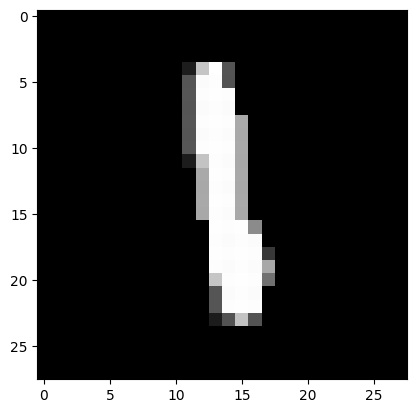
\includegraphics[width=0.6\linewidth]{images/neural_network/digital_twin_784_input.png}
    \caption{784 pixels image.}
    \label{fig:mnist_image}
\end{figure}

The input image is then converted into 8-bit values, and an average pooling operation is applied to reduce the image size from 28x28 pixels to 14x14 pixels. 

The result of this pooling is shown in Figure \ref{fig:pooled_image}. This downsampling helps reduce the image complexity while preserving essential features.

\begin{figure}[!h]
    \centering
    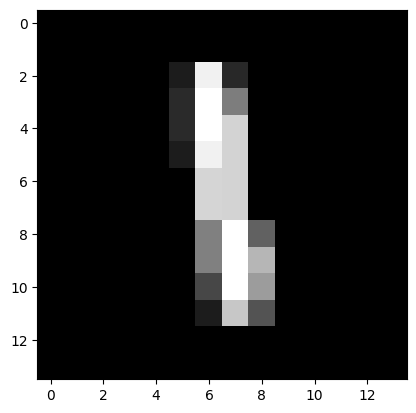
\includegraphics[width=0.6\linewidth]{images/neural_network/digital_twin_196_input.png}
    \caption{196 pixels pooled image.}
    \label{fig:pooled_image}
\end{figure}

The pooled image is flattened into a single vector, with each pixel value in 8-bit precision, and this vector is used as input for verification in ModelSim. The same 8-bit precision vector is also provided to the neural network implemented in Python. The following results are shown below for comparison:

\begin{itemize}
    \item \textbf{Hidden Dense Layer Output:} \\
    The following values represent the outputs from the hidden dense layer:

    \begin{tabular}{|c|c|c|c|c|c|c|c|c|c|}
    \hline
    -3901 & 1093 & 12652 & -15824 & 17194 & 2749 & 7575 & 21018 & 16200 & -5915 \\
    \hline
    15908 & -33645 & 1273 & -1952 & 18383 & -861 & -5374 & 70 & 15622 & 587 \\
    \hline
    22639 & 33790 & 10544 & 10283 & -38405 & 20328 & 11178 & -9242 & -3343 & 23940 \\
    \hline
    10088 & 15426 &  &  &  &  &  &  &  &  \\
    \hline
    \end{tabular}

    \item \textbf{Hidden ReLU Layer Output:} \\
    After applying the ReLU activation function to the hidden dense layer outputs, we get the following:

    \begin{tabular}{|c|c|c|c|c|c|c|c|c|c|}
    \hline
    0 & 1093 & 12652 & 0 & 17194 & 2749 & 7575 & 21018 & 16200 & 0 \\
    \hline
    15908 & 0 & 1273 & 0 & 18383 & 0 & 0 & 70 & 15622 & 587 \\
    \hline
    22639 & 33790 & 10544 & 10283 & 0 & 20328 & 11178 & 0 & 0 & 23940 \\
    \hline
    10088 & 15426 &  &  &  &  &  &  &  &  \\
    \hline
    \end{tabular}
    
    \item \textbf{Output Dense Layer Output:} \\
    The outputs from the output dense layer are as follows:

    \begin{tabular}{|c|c|c|c|c|c|}
    \hline
    -5056117 & 2074036 & -1236868 & -459815 & -1518830 & -2264880 \\
    \hline
    -2325566 & -2609297 & 246759 & -3254669 & & \\
    \hline
    \end{tabular}
    
    \item \textbf{Final Output ReLU Layer Output:} \\
    The output after applying the ReLU activation to the final layer:

    \begin{tabular}{|c|c|c|c|c|c|c|c|c|c|}
    \hline
    0 & 2074036 & 0 & 0 & 0 & 0 & 0 & 0 & 246759 & 0 \\
    \hline
    \end{tabular}

    \item \textbf{Predicted Digit:} \\
    The final predicted digit from the neural network is: 1

\end{itemize}

These results are based on the flattened input data and show the outputs at each stage of the neural network. The final output, after passing through the dense and ReLU layers, is compared with the predicted digit, which, in this case, is '1'. This predicted value is consistent with the label shown in the MNIST dataset for the chosen example image.

By comparing these results with the ModelSim simulation, we verify the correctness and consistency of the hardware implementation against the digital twin.

\subsection{ModelSim Simulation}

Figure \ref{fig:modelsim_temporization} shows the timing diagram of the forward logic finite state machine (FSM) for the input described in the previous section: a '1' represented by 196 pixels in 8-bit precision. The FSM is triggered by a start signal, which indicates the beginning of the computation process. Once the FSM completes its operations, the "done" signal is asserted to indicate that the computation has finished.

The expected output is displayed in the waveform, showing the result of the FSM execution for this specific input. The output signal corresponds to the computed result after processing the 8-bit input data.

In the next section, the internal outputs from the various stages of the computation are presented in more detail.

\begin{figure}[!h]
    \centering
    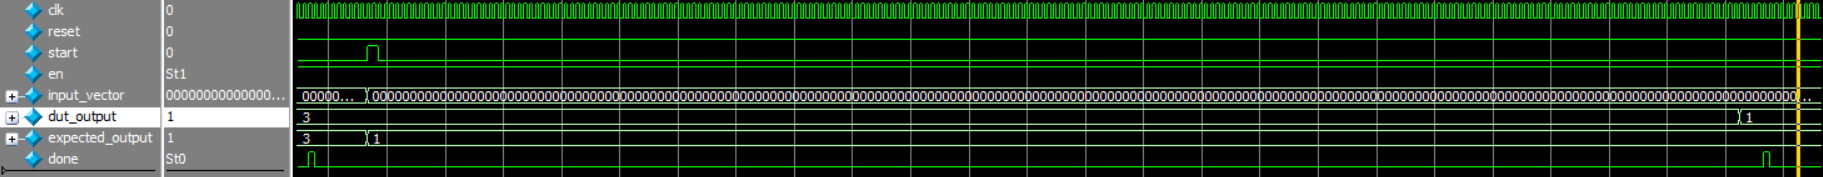
\includegraphics[width=1\linewidth]{images/neural_network/modelsim_NN_waveform.png}
    \caption{Modelsim temporization.}
    \label{fig:modelsim_temporization}
\end{figure}

\subsection{Log Results from ModelSim}

In this section, the intermediate outputs of the neural network are shown. The results are captured in the testbench using the \texttt{write} function in a \texttt{for} loop, which is executed after each \texttt{done} signal is asserted by each layer of the network. This allows for capturing the outputs of the layers as they complete their computations.

The intermediate results are shown in Figure \ref{fig:modelsim_logs}. These results represent the state of the network after each layer's computation, helping to verify the functionality and correctness of the forward pass.

\begin{figure}[h]
    \centering
    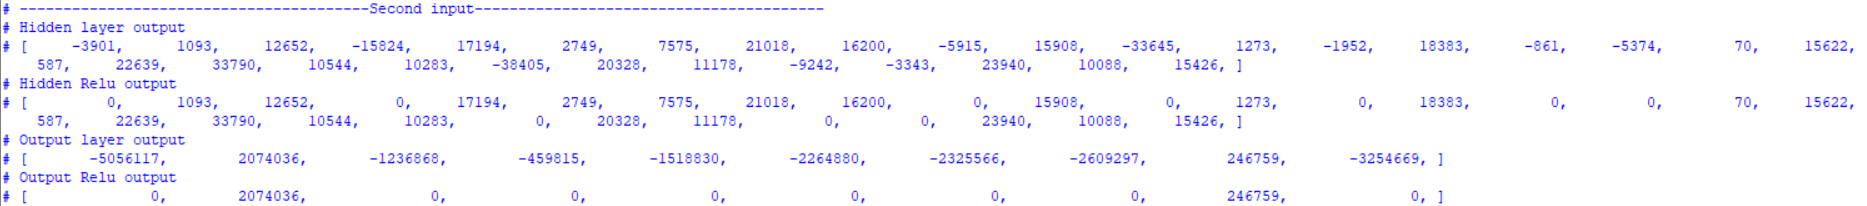
\includegraphics[width=1\textwidth]{images/neural_network/modelsim_NN_logs.png}
    \caption{Log results showing the intermediate outputs from each layer of the neural network.}
    \label{fig:modelsim_logs}
\end{figure}

As it can be seen, the outputs coincide with those found in the digital twin. It is important to note that for this type of simulation, it is interesting to observe the functioning of the system with a second input, in order to verify if all the neurons work as described and if the MAC is properly reset after the completion of a prediction. This is why Figure \ref{fig:modelsim_logs} represents the output as "second input." The first input, which is not shown here for clarity, is a different input used earlier in the simulation.

\chapter{Graphic Interface Design}\label{chap:graphic_interface_design}
The \textbf{Graphic Interface} sub-system performs the following tasks:

\begin{itemize}
    \item It manages the ILI9341 TFT display controller and continuously updates what is shown on the display, by fetching pixels from a frame buffer memory in a circular manner.
    \item It drives the AD7843 touch screen digitizer in order to obtain the location of the touched point on the screen.
    \item It gets the coordinates of the touched location and updates the image shown on the display by adding a white pixel at those coordinates. If the touched point lies inside a given drawing area, it also adds that white pixel to a special buffer memory, that contains the inputs of the neural network.
    \item It can load on the frame memory constant frames stored inside a ROM, so that the default background image on the display can be customized.
\end{itemize}

The Quartus block of this sub-system is shown in Fig. \ref{fig:graphic_block}

\begin{figure}[!h]
    \centering
    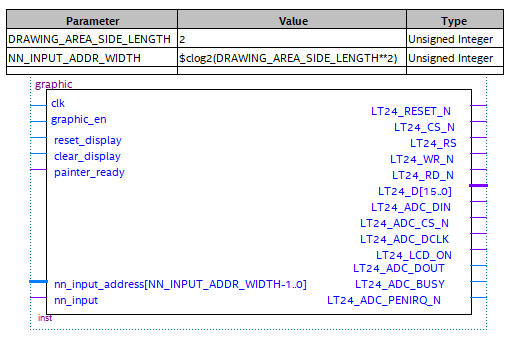
\includegraphics[width=0.6\linewidth]{images/graphic_interface_design/graphic_interface_block.png}
    \caption{Quartus block of graphic interface sub-system.}
    \label{fig:graphic_block}
\end{figure}

The interface of the graphic block is illustrated in Tables \ref{tab:graphic_block_interface} and \ref{tab:graphic_block_lt24_interface}.

\begin{table}[!h]
\renewcommand{\arraystretch}{1.5}
\centering
\begin{tabular}{|c|c|c|p{60mm}|}
\hline
\textbf{Port name}   & \textbf{Size}           & \textbf{I/O} & \multicolumn{1}{c|}{\textbf{Description}} \\ \hline
clk                  &  1                      & In & Global clock   \\ \hline
graphic\_en          &  1                      & In & Enable (active high)        \\ \hline
reset\_display       &  1                      & In & Reset all the drivers and the LCD display (active high)                     \\ \hline
clear\_display       &  1                      & In & Clear the drawn content of the display and load a default constant frame (active high)                      \\ \hline
painter\_ready       &  1                      & Out & Signals when the painter has finished to load a constant frame or to draw a touched pixel and it is ready to receive new commands (active high)                     \\ \hline
nn\_input\_address   &  NN\_INPUT\_ADDR\_WIDTH & In & Read address to the neural network inputs memory                      \\ \hline
nn\_input            &  1                      & Out & Output of the neural network inputs memory at the read address location                     \\ \hline

\end{tabular}
\label{tab:graphic_block_interface}
\caption{Internal interface of the graphic block.}
\end{table}

\begin{table}[!h]
\renewcommand{\arraystretch}{1.5}
\centering
\begin{tabular}{|c|c|c|p{60mm}|}
\hline
\textbf{Port name}   & \textbf{Size}    & \textbf{I/O}  & \multicolumn{1}{c|}{\textbf{Description}} \\ \hline
LT24\_RESET\_N       &  1               &  Out          &  LCD hardware reset (active low)                   \\ \hline
LT24\_CS\_N          &  1               &  Out          &  LCD chip select (active low)                   \\ \hline
LT24\_RS             &  1               &  Out          &  LCD command/data selector                    \\ \hline
LT24\_WR\_N          &  1               &  Out          &  LCD write enable                    \\ \hline
LT24\_RD\_N          &  1               &  Out          &  LCD read enable                    \\ \hline
LT24\_D              &  16              &  Out          &  LCD parallel data bus                    \\ \hline
LT24\_ADC\_DIN       &  1               &  Out          &  ADC serial data input                   \\ \hline
LT24\_ADC\_CS\_N     &  1               &  Out          &  ADC chip select (active low)                    \\ \hline
LT24\_ADC\_DCLK      &  1               &  Out          &  ADC data clock                    \\ \hline
LT24\_ADC\_DOUT      &  1               &  In           &  ADC serial data output                    \\ \hline
LT24\_ADC\_BUSY      &  1               &  In           &  ADC busy flag (active high)                    \\ \hline
LT24\_ADC\_PENIRQ\_N &  1               &  In           &  ADC touch interrupt request                    \\ \hline
LT24\_LCD\_ON        &  1               &  Out          &  LCD backlight enable (active high)                    \\ \hline


\end{tabular}
\label{tab:graphic_block_lt24_interface}
\caption{Interface of the graphic block with the LT24 display.}
\end{table}

A description of the parameters of the sub-system is shown in Table \ref{tab:graphic_interface_param}.

\begin{table}[!h]
\renewcommand{\arraystretch}{1.5}
\centering
\begin{tabular}{|c|c|p{20mm}|}
\hline
\textbf{Parameter}          & \textbf{Default value} & \multicolumn{1}{c|}{\textbf{Description}} \\ \hline
DRAWING\_AREA\_SIDE\_LENGTH & 224                    &  Length in pixels of the square drawing area of the display, whose pixels will be sent as input of the neural network. Its squared value also represents the size of the neural network inputs memory                    \\ \hline
NN\_INPUT\_ADDR\_WIDTH      & $\log_2(\text{DRAWING\_AREA\_SIDE\_LENGTH**2})$ & Address width of the neural network inputs memory                     \\ \hline
\end{tabular}
\label{tab:graphic_interface_param}
\caption{Parameters of the graphic interface block.}
\end{table}

A schematic view of the block design of the graphic interface is shown in Fig. \ref{fig:graphic_interface_diagram}.

\begin{figure}[!h]
\centering
\resizebox{1\linewidth}{!}{%
\begin{circuitikz}
\tikzstyle{every node}=[font=\footnotesize]
\draw  (2.5,5.25) rectangle  node {\normalsize Touchscreen driver} (6.25,2.75);
\draw  (8.75,5.25) rectangle  node {\normalsize Painter} (12.5,2.75);
\draw  (15,5.25) rectangle  node {\normalsize Frame RAM} (18.75,2.75);
\draw  (15,9) rectangle  node {\normalsize NN inputs memory} (18.75,6.5);
\draw  (21.25,5.25) rectangle  node {\normalsize Graphic controller} (25,2.75);
\draw  (21.25,1.5) rectangle  node {\normalsize LCD driver} (25,-1);
\draw [ dashed] (27.5,1.5) rectangle  node {\normalsize ILI9341}  (30,-1);
\draw [ dashed] (2.5,0.25) rectangle  node {\normalsize AD7843}  (6.25,-2.25);
\draw  (8.75,0.25) rectangle  node {\normalsize Frame ROM} (12.5,-2.25);
\draw [->, >=Stealth] (6.25,4) -- (8.75,4)node[pos=0.5,above, fill=white]{ADC Result};
\draw (11.25,8.5) to[short] (11.25,5.25);
\draw [->, >=Stealth] (25,0.25) -- (27.5,0.25);
\draw [->, >=Stealth] (11.25,8.5) -- (15,8.5)node[pos=0.5,above, fill=white]{write address};
\draw [->, >=Stealth] (18.75,7.75) -- (21.25,7.75)node[pos=0.5,above, fill=white]{nn\_input};
\draw [->, >=Stealth] (22.5,2.75) -- (22.5,1.5)node[pos=0.5,left, fill=white]{pixel value};
\draw [->, >=Stealth] (23.75,1.5) -- (23.75,2.75)node[pos=0.5,right, fill=white]{driver ready};
\draw [->, >=Stealth] (5,0.25) -- (5,2.75)node[pos=0.5,right, fill=white]{ADC Response};
\draw [->, >=Stealth] (3.75,2.75) -- (3.75,0.25)node[pos=0.5,left, fill=white]{ADC Request};
\draw [->, >=Stealth] (10,2.75) -- (10,0.25)node[pos=0.5,left, fill=white]{address};
\draw [->, >=Stealth] (11.25,0.25) -- (11.25,2.75)node[pos=0.5,right, fill=white]{pixel value};
\draw [->, >=Stealth] (12.5,3.25) -- (15,3.25)node[pos=0.5,above, fill=white]{write address};
\draw [->, >=Stealth] (18.75,4.75) -- (21.25,4.75)node[pos=0.5,above, fill=white]{read pixel value};
\draw [->, >=Stealth] (21.25,3.25) -- (18.75,3.25)node[pos=0.5,above, fill=white]{read address};
\draw [->, >=Stealth] (17.5,10.25) -- (17.5,9)node[pos=0.5,right, fill=white]{nn\_input\_address};
\draw [->, >=Stealth] (12.5,4.75) -- (15,4.75);
\draw (12,5.25) to[short] (12,7);
\draw [->, >=Stealth] (12,7) -- (15,7)node[pos=0.5,above, fill=white]{pixel value};
\draw (7.25,3.75) to[short] (7.75,4.25);
\draw (9.75,1.25) to[short] (10.25,1.75);
\draw (3.5,1.25) to[short] (4,1.75);
\draw (4.75,1.25) to[short] (5.25,1.75);
\draw (19.75,3) to[short] (20.25,3.5);
\draw (13.5,3) to[short] (14,3.5);
\draw (22.25,2) to[short] (22.75,2.5);
\draw (12.25,8.25) to[short] (12.75,8.75);
\draw (17.25,9.75) to[short] (17.75,10.25);
\draw (26,0) to[short] (26.5,0.5);
\draw [->, >=Stealth] (9,7.75) -- (9,5.25)node[pos=0.5,left, fill=white]{clear\_display};
\draw [->, >=Stealth] (8.25,8.5) -- (7.5,8.5)node[pos=0.5,above, fill=white]{painter\_ready};
\draw (9,7.75) to[short] (7.5,7.75);
\draw (8.25,8.5) to[short] (10,8.5);
\draw (10,8.5) to[short] (10,5.25);
\draw (7.75,8.5) to[short] (9.75,8.5);
\node [font=\footnotesize] at (26.25,-1.75) {ILI9341 command interface};
\node [font=\footnotesize] at (13.75,5.5) {write pixel value};
\end{circuitikz}
}%

\label{fig:graphic_interface_diagram}
\caption{Schematic view of the graphic interface block design.}
\end{figure}

As we can see, the \textbf{painter} is at the core of the sub-system. It loads constant frames stored inside a frame ROM to a frame RAM that is used as a buffer memory between the painter itself and the \textbf{graphic controller}, which - as will be explained in Sec. \ref{sec:graphic_controller} - must operate at a slower speed. The graphic controller reads from the frame RAM and sends each pixel to the \textbf{LCD driver}, which communicates with the LT24 display controller (the \textbf{ILI9341}) in order to update the respective pixel. Given that the graphic controller continuously reads the frame RAM in a circular array manner and repeatedly refresh the display pixels at the maximum allowed ILI9341 frequency, the frame updates are unnoticeable to the user, who experiences smooth transitions. Whenever the screen is touched, the touchscreen digitizer, the \textbf{AD7843}, sends an interrupt request to the touchscreen driver, which communicates with the ADC in order to initialize an acquisition procedure and subsequently obtain the sampled and digitized touch location from the ADC itself. This information is sent to the painter, which elaborates it and adds a white pixel to the frame RAM at the received coordinates. If the touched location lies inside a certain drawing area (a square area with side length equal to DRAWING\_AREA\_SIDE\_LENGTH and with the top left corner aligned with the display origin), the painter also writes the touched pixel at the corresponding address inside the \textbf{NN input memory}, which can be successively read to retrieve the input data for the neural network.

The specific features and operation modes of each block will be analyzed in the following sections.

\section{LT24 LCD Driver}\label{sec:lt24_lcd_driver}
The LT24 LCD driver directly communicates with the ILI9341 controller used on the Terasic LT24 board to drive the display through the signals listed in Table \ref{tab:graphic_block_lt24_interface}.

\begin{figure}[!h]
    \centering
    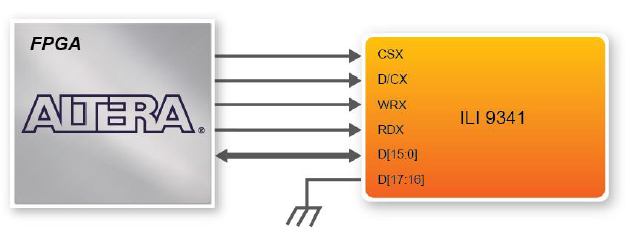
\includegraphics[width=1\linewidth]{images/graphic_interface_design/LT24_LCD_driver/ili9341_connections.png}
    \caption{Signals of the LCD driver connected to the FPGA}
    \label{fig:ili9341_connections}
\end{figure}

The LCD features a 240x320 pixel resolution. The ILI9341 controller is hardware programmed on the LT24 board to use the 8080-I system 16-bit parallel bus interface, where colors are encoded with a RGB 5-6-5 code (5-bit for red, 6-bit for blue and 5-bit for green), enabling a 65K wide range of colors. However, in our system only two colors are needed, black (all zeros) and white (all ones), in order to significantly reduce the size of the frames memories, because each pixel can be encoded with only one bit. The write cycle sequence of the parallel bus protocol is shown in Fig. \ref{fig:8080_protocol}.

\begin{figure}
    \centering
    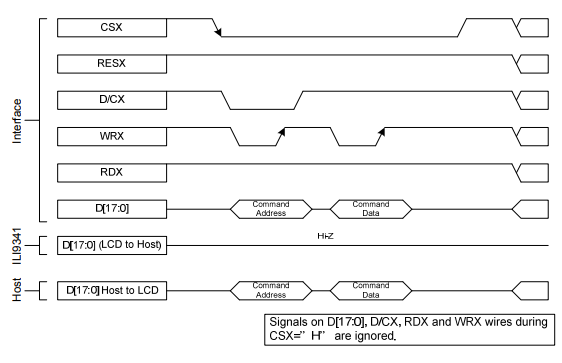
\includegraphics[width=1\linewidth]{images/graphic_interface_design/LT24_LCD_driver/8080_protocol.png}
    \caption{ILI9341 8080-I 16-bit parallel bus write cycle sequence.}
    \label{fig:8080_protocol}
\end{figure}

CSX is a low active chip select pin and, given that we want to drive only one ILI9341 display controller, it is always kept active. D/CX is Data or Command selection pin. When D/CX = 1, data is selected and the parallel bus content D[15:0] is interpreted as a RGB 5-6-5 pixel value. When D/CX = 0, command is selected and the parallel bus content is interpreted as a command. WRX is a write signal and the ILI9341 reads data at its rising edge. RDX is a read signal and the FPGA reads data at the rising edge. However, in this application the communication between the FPGA and the ILI9341 is needed only in write mode and a read sequence is never initialized. For this reason, the RDX signal (active low) is always kept at VCC.

From the \href{https://cdn-shop.adafruit.com/datasheets/ILI9341.pdf}{datasheet} of ILI9341 we were able to obtain the maximum allowed frequency of WRX signal, hence the maximum frequency of a write cycle, which is approximately 15 MHz. This is because a full write cycle is comprised of a certain amount of time while WRX is kept low plus some more time while WRX is kept high, as shown in Fig.\ref{fig:8080_protocol}. Therefore, the LT24 LCD driver cannot be driven with the global 50 MHz clock, but, thanks to an enable control, it is slowed down to 25 MHz and WRX can be toggled at most every clock period. For this reason, a full write cycle sequence lasts exactly 2 clock cycles.

In order to correctly set the display up, a precise reset procedure and a certain initialization commands sequence must be applied to the display upon reset, as shown in Fig. \ref{fig:ili9341_initialization_seq}.

\begin{figure}[!h]
\centering
\resizebox{1\linewidth}{!}{% Reduce size of everything
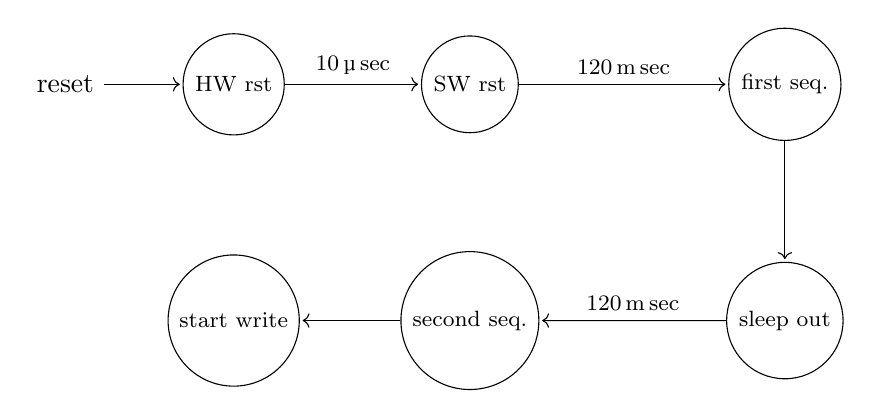
\begin{tikzpicture}[shorten >=1pt, node distance=3cm, on grid,
                    initial distance=1cm, initial text=reset,
                    bend angle=45,
                    every state/.style={font=\footnotesize}]
    %\draw[help lines] (0,-5) grid (10,10);

   \node[state,initial] (reset_low)                             {HW rst};   
   \node[state]         (sw_reset)    [right=of reset_low]      {SW rst}; 
   \node[state]         (first_init)  at (7, 0) {first seq.}; 
   \node[state]         (exit_sleep)  [below=of first_init]     {sleep out};
   \node[state]         (second_init) at (3, -3) {second seq.};
   \node[state]         (start_write) [left=of second_init]     {start write};

   % Define transitions
   \path[->,every node/.style={font=\footnotesize}]
    (reset_low)   edge      node [above] {\SI{10}{\micro\sec}}  (sw_reset)
    (sw_reset)    edge      node [above] {\SI{120}{\milli\sec}} (first_init)
    (first_init)  edge      node []      {}                     (exit_sleep)
    (exit_sleep)  edge      node [above] {\SI{120}{\milli\sec}} (second_init)
    (second_init) edge      node []      {}                     (start_write);
          %edge [loop above] node {index!=IN\_SIZE-1} ();
    
\end{tikzpicture}
}
\caption{ILI9341 initialization sequence}
\label{fig:ili9341_initialization_seq}
\end{figure}

As we can see, the initialization sequence starts with an hardware reset (by pulling down the pin LT24\_RESET\_N) which must last at least \SI{10}{\micro\sec}, as specified in the datasheet. Afterwards, a software reset command must be given and we must wait at least \SI{120}{\milli\sec} before firing the next command. Subsequently, we can start with the first initialization commands sequence, which is used to set some LCD power settings, declare the pixel format (RGB 5-6-5) and to define the way the ILI9341 accesses its own memory (this is necessary to set the screen in landscape mode). After that, we can send a command that makes the ILI9341 exit the sleep mode, which again requires a wait time of at least \SI{120}{\milli\sec}, and then we can conclude with the second initialization commands sequence, which is used to set the column range from 0 to 319 and the row range from 0 to 239, so that the display can be used in landscape mode (normally it would be used in portrait mode, but for this application it was not much comfortable to use). Eventually, a start memory write command is sent and after that we can send data words containing the RGB 5-6-5 code of each pixel given in increasing order, from the top left corner to the bottom right corner: the ILI9341 controller will automatically increase the address of the current pixel after each write cycle and it will wrap back to 0 as soon as the maximum address (239, 319) is reached; this way we can continuously update the LCD display internal RAM, without having to feed any other command. The sequence of parallel bus data from the start memory write is shown in Fig. \ref{fig:pixel_sequence}.

\begin{figure}[!h]
    \centering
    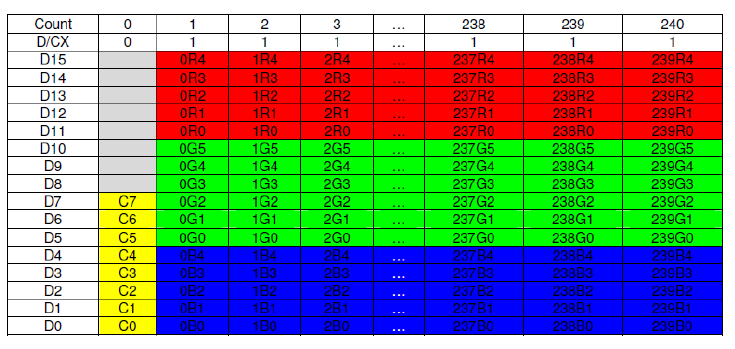
\includegraphics[width=1\linewidth]{images/graphic_interface_design/LT24_LCD_driver/write_pixels_sequence.png}
    \caption{ILI9341 start memory write command and pixels RGB 5-6-5 code sequence.}
    \label{fig:pixel_sequence}
\end{figure}

All the initialization sequence commands and respective payload data are stored inside a LUT, which is accessed sequentially during the initialization sequence by the LT24 LCD driver.

\begin{figure}[!h]
    \centering
    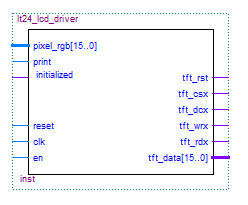
\includegraphics[width=0.5\linewidth]{images/graphic_interface_design/LT24_LCD_driver/lcd_driver_quartus_block.png}
    \caption{LT24 LCD driver Quartus block}
    \label{fig:lcd_driver_quartus_block}
\end{figure}

As soon as the driver initialization sequence is complete, the output pin \textbf{initialized} is pulled up (see Fig. \ref{fig:lcd_driver_quartus_block}), in order to notify the \textbf{graphic controller} (see Sec. \ref{sec:graphic_controller}) that the driver is now ready to receive ordered pixel codes and forward them to the display controller. When the input pin \textbf{print} is set high, the LT24 LCD driver samples the value of \textbf{pixel\_rgb[15..0]} and it starts a write cycle sequence in data mode with the ILI9341, sending the received RGB code. After exactly two clock cycles, the write cycle sequence is complete and the driver can accept a new pixel to print. All the previously described temporizations are performed by means of counters.

\subsection{Display Orientation}

The orientation of the display in the final application is the one shown in Fig. \ref{fig:lcd_orientation}.

\begin{figure}[!h]
    \centering
    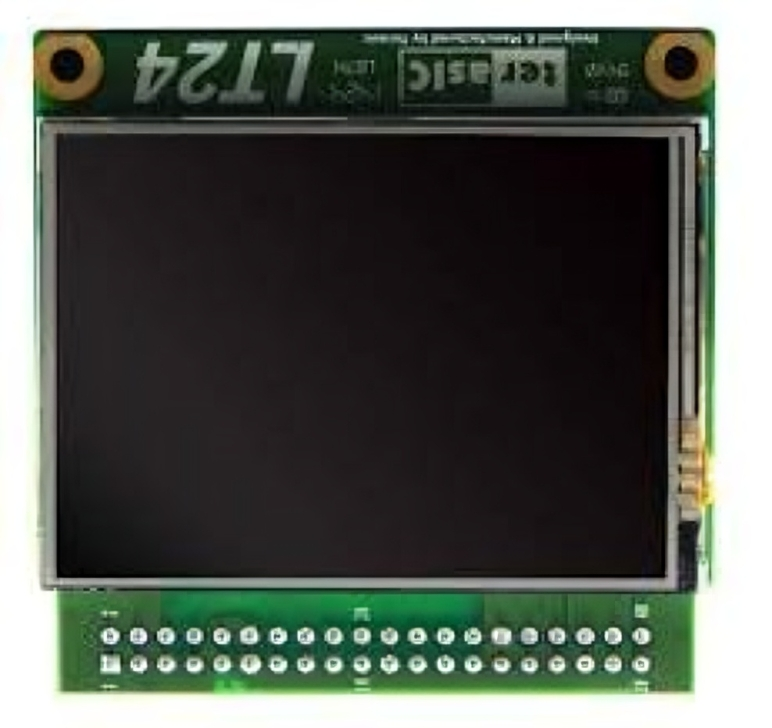
\includegraphics[width=0.5\linewidth]{images/graphic_interface_design/LT24_LCD_driver/LCD_orientation.png}
    \caption{LT24 display final orientation.}
    \label{fig:lcd_orientation}
\end{figure}

The first pixel is at the top left and the last at the bottom right. The X axis goes from left to right and the Y axis goes from top to bottom. This orientation is the most comfortable to use with the DE10-Lite, because of the position of the GPIO header on which the LT24 board is connected. The same considerations apply to the touchscreen driver, which also has inverted axes compared to the default portrait orientation (see Sec. \ref{sec:touchscreen_driver}).

\subsection{Modelsim Simulation}
This driver has been simulated in Modelsim and we could verify that the initialization sequence and the 8080-I parallel protocol followed, as shown in Fig. \ref{fig:init_sim} and \ref{fig:8080_sim}.

\begin{figure}[!h]
    \centering
    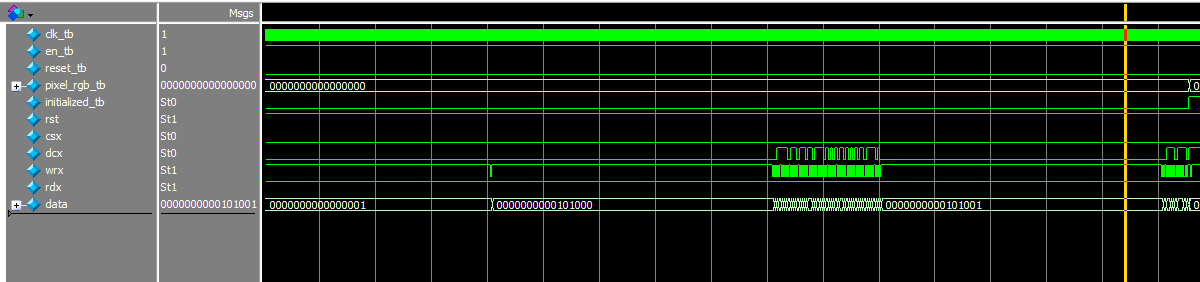
\includegraphics[width=1\linewidth]{images/graphic_interface_design/LT24_LCD_driver/initialization_simulation.png}
    \caption{LT24 LCD driver initialization sequence simulation in Modelsim.}
    \label{fig:init_sim}
\end{figure}

\begin{figure}[!h]
    \centering
    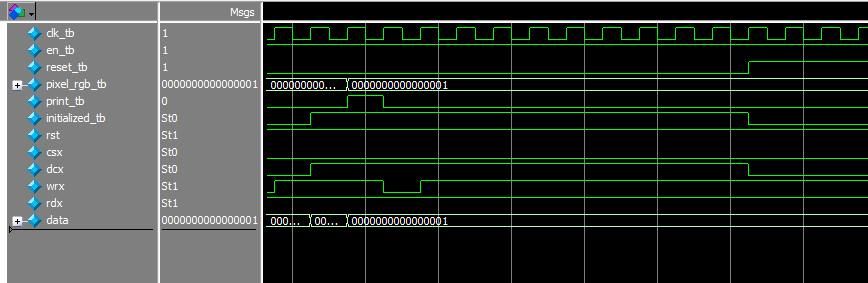
\includegraphics[width=1\linewidth]{images/graphic_interface_design/LT24_touchscreen_driver/8080_protocol_simulation.png}
    \caption{LT24 LCD driver 8080-I parallel communication protocol simulation in Modelsim.}
    \label{fig:8080_sim}
\end{figure}

\section{LT24 Graphic Controller}\label{sec:graphic_controller}
The task performed by the LT24 graphic controller is to cyclically read each pixel from the frame RAM, in which is stored an image of resolution 240x320 pixel of 1-bit each, it converts it into a RGB 5-6-5 code (0x0000 if the pixel is 0 or 0xFFFF is the pixel is 1) and it sends it to the LT24 LCD driver while activating the print input, as mentioned in the previous section. The graphic controller is feeded with the same clock as the LT24 LCD driver, therefore, after exactly two clock cycles, the controller can send the next pixel to the driver. While waiting for the driver, the graphic controller fetches the following pixel from the RAM.

\begin{figure}[!h]
    \centering
    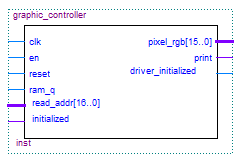
\includegraphics[width=0.5\linewidth]{images/graphic_interface_design/graphic_controller/graphic_controller_quartus_block.png}
    \caption{LT24 graphic controller Quartus block.}
    \label{fig:graphic_controller_quartus_block}
\end{figure}

The graphic controller starts to read the RAM only when the driver has completed the initialization sequence. (\textbf{driver\_initialized} is high).

The state flow of the graphic controller is shown in Fig. \ref{fig:graphic_controller_fsm}.

\begin{figure}[!h]
\centering
\resizebox{1\linewidth}{!}{% Reduce size of everything
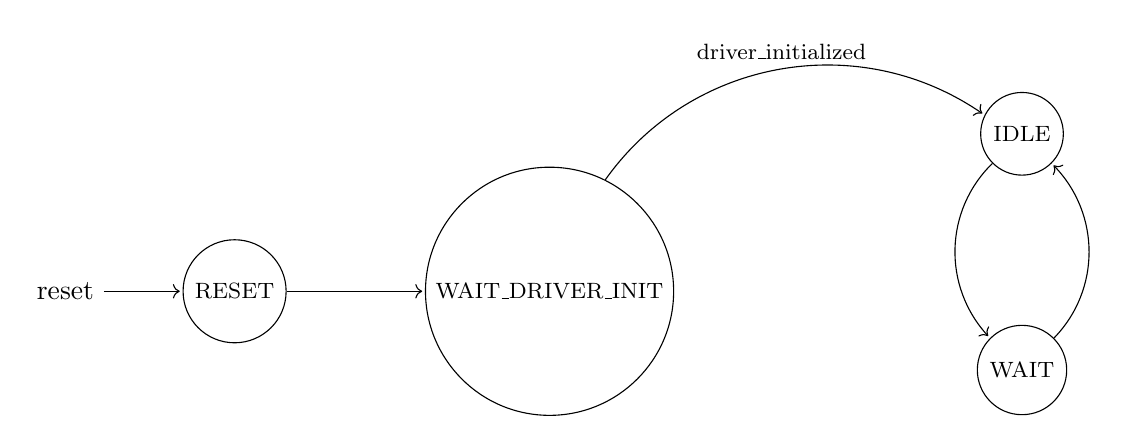
\begin{tikzpicture}[shorten >=1pt, node distance=3cm, on grid,
                    initial distance=1cm, initial text=reset,
                    bend angle=45,
                    every state/.style={font=\footnotesize}] 
    %\draw[help lines] (0,-5) grid (10,10);

   \node[state,initial] (reset) {RESET};   
   \node[state] (wait_driver) at (4, 0) {WAIT\_DRIVER\_INIT}; 
   \node[state] (idle) at (10, 2) {IDLE}; 
   \node[state] (wait) [below=of idle] {WAIT};

   % Define transitions
   \path[->,every node/.style={font=\footnotesize}]
    (reset)       edge              node {} (wait_driver)
    (wait_driver) edge [bend left]  node [above] {driver\_initialized} (idle)
    (idle)        edge [bend right] node {} (wait)
    (wait)        edge [bend right] node {} (idle);
    
\end{tikzpicture}
}
\caption{LT24 graphic controller state flow.}
\label{fig:graphic_controller_fsm}
\end{figure}

In the IDLE state, the graphic controller fetches the output of the frame RAM at the current address, which starts from 0. In the WAIT state, the graphic controller pulls up the \texttt{print} signal, signaling to the LT24 LCD driver that the new pixel is ready, and also enables the frame RAM address counter, which will be increased at the end of the current clock period: this way, at the next clock's rising edge (at the end of the IDLE state) the RAM will return the content of the adjacent memory location, which will be fed to the LCD driver, which, in the mean time, has completed one full write cycle sequence. When the RAM address counter overflows, it wraps back to 0 and the frame RAM is read again.

It is important to notice that the ILI9341 controller expects the pixels given in row order, i.e. it starts writing the pixels of row 0 first (from column 0 to column 319) and ends with the pixels of row 239. The graphic controller must feed the pixel colors in the same order. For this reason, the frame RAM is designed as a 1D flattened matrix of $240\times320=76800$ 1-bit pixels organized as a concatenation of the rows that form a frame. Therefore, the first element of the RAM will represent the pixel of coordinates (0, 0) and the last will represent the pixel of coordinates (239, 319).

\section{LT24 Touchscreen Driver}\label{sec:touchscreen_driver}
The task performed by the LT24 touchscreen driver is to wait for a touch event on the screen and send a request to the ADC mounted on the LT24 board to obtain the coordinates of the touched point. These obtained values are then sent to the painter module (see Sec \ref{sec:painter}).

\begin{figure}[!h]
    \centering
    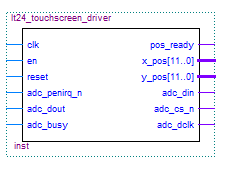
\includegraphics[width=0.5\linewidth]{images/graphic_interface_design/LT24_touchscreen_driver/touchscreen_driver_quartus_block.png}
    \caption{LT24 touchscreen driver Quartus block}
    \label{fig:touchscreen_driver_quartus_block}
\end{figure}

The mounted ADC is the AD7483 from Analog Device and it has a resolution of 12 bits. It measures resistance variations of the resistive touch screen layer, which lies on top of the screen. To obtain the coordinates from the ADC, users need to monitor the interrupt signal LT24\_ADC\_PENIRQ\_N coming out of the ADC first. This signal is normally high, thanks to a pullup resistor mounted on the LT24. When the touch screen connected to the
ADC is triggered via a pen or finger, the LT24\_ADC\_PENIRQ\_N output goes low and and the touchscreen driver instructs a control word to be written to the ADC via the serial port interface LT24\_ADC\_DIN. The control word provided to the ADC via the DIN pin is described in Table \ref{tab:adc_control_word}. It controls the conversion start, channel addressing, ADC conversion resolution, configuration, and power-down of the ADC.

\begin{table}[!h]
\caption{Control register bit function description.}
\label{tab:adc_control_word}
\renewcommand{\arraystretch}{1.5}
\centering
\begin{tabular}{|cccccccc|}
\hline
\textbf{MSB}                     &                         &                         &                         &                           &                              &                          & \textbf{LSB} \\ \hline
\multicolumn{1}{|c|}{S} & \multicolumn{1}{c|}{A2} & \multicolumn{1}{c|}{A1} & \multicolumn{1}{c|}{A0} & \multicolumn{1}{c|}{MODE} & \multicolumn{1}{c|}{SER/$\overline{\text{DFR}}$} & \multicolumn{1}{c|}{PD1} & PD0 \\ \hline
\end{tabular}

\medskip
\begin{tabular}{|c|c|p{120mm}|}
\hline
\textbf{Bit} & \textbf{Mnemonic} & \multicolumn{1}{c|}{\textbf{Comment}} \\ \hline
7            & S                 &  Start bit. The control word starts with the first high bit on DIN. A new control word can startevery 15th DCLK cycle when in the 12-bit conversion mode, or every 11th DCLK cycle when in the 8-bit conversion mode.               \\ \hline
6-4          & A2-A0             & Channel select bits. these three address bits, along with SER/$\overline{\text{DFR}}$ bit, control the setting of the multiplexer input, switches and reference inputs.                 \\ \hline
3            & MODE              & 12-bit/8-bit conversion select bit. This bit controls the resolution of the following conversion. With 0 in this bit, the conversion has a 12-bit resolution, or with 1 in this bit, the conversion has a 8-bit resolution.                 \\ \hline
2            & SER/$\overline{\text{DFR}}$           & Single-Ended/Differential Reference select bit. Along with bits A2-A0, this bit controls the setting of the multiplexer input, switches and reference inputs.                 \\ \hline
1-0          & PD1,PD0           & Power management bits. These two bits decode the power-down mode of the AD7843.                 \\ \hline
\end{tabular}
\end{table}

In order to start the ADC conversion, different control sequences are available and described in the \href{https://www.analog.com/media/en/technical-documentation/data-sheets/AD7843.pdf}{datasheet}. However, for our application, the fastest one was chosen, since it allows to reach the maximum throughput reachable by the ADC. With this sequence, it is possibile to complete two subsequent conversions (one the the X coordinate and one for the Y coordinate) in only 36 DCLK cycles. This sequence is illustrated in Fig \ref{fig:ad7483_sequence}.

\begin{figure}[!h]
    \centering
    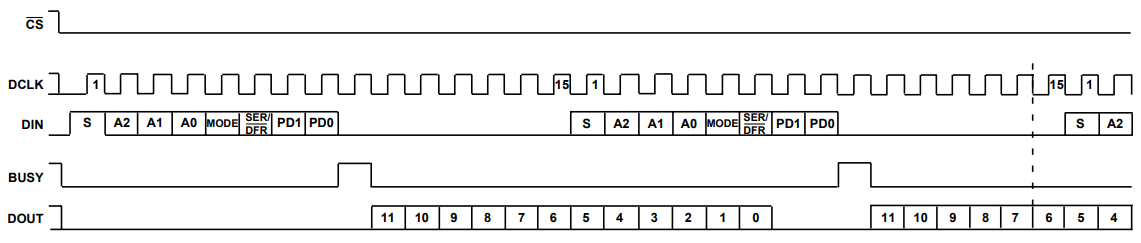
\includegraphics[width=1\linewidth]{images/graphic_interface_design/LT24_touchscreen_driver/ad7843_sequence.png}
    \caption{AD7483 15 DCLKS per cycle conversion sequence.}
    \label{fig:ad7483_sequence}
\end{figure}

Notice that the DCLK signal is provided by the touchscreen driver itself and it must not exceed 2 MHz.

As we can see from Fig. \ref{fig:ad7483_sequence}, as soon as the interrupt signal is received, the touchscreen driver can send the control word to the ADC to instruct it to start the acquisition and digitalization of the X coordinate of the touched point. After that, exactly one DCLK cycle is required to the ADC to acquire the input analog voltage and then it starts with the conversion: the 12 bits are returned serially on the LT24\_ADC\_DOUT port, from where they are sampled and deserialized, thanks to a 12-bit buffer register. Before the X conversion has ended, after a total number of 15 DCLK cycles, the driver can already start to instruct the ADC with a different control word, which enables the readout of the Y coordinate of the touched location. After the 8 bits of the control word, 1 DCLK cycle is used for the acquisition and then the serialized Y conversion output is sent on the DOUT port. When both X and Y values have been obtained, the touchscreen driver terminates the request and disables the LT24\_ADC\_CS\_N output pin. Notice that during the 15 DCLK cycle conversion, we assume that the location of the touched point on the screen does not change, allowing us to obtain the X and Y coordinates of the same point. This assumption can be easily considered as true, as long as the operation frequency of the ADC DCLK is fast enough, see Sec. \ref{sec:adc_clock}.

\medskip
The control words used for the two types of conversions are the following:

\begin{table}[!h]
\renewcommand{\arraystretch}{1.5}
\centering
\begin{tabular}{c|c|c|}
\cline{2-3}
                                             & \textbf{X conversion} & \textbf{Y conversion} \\ \hline
\multicolumn{1}{|c|}{\textbf{Control words}} & 10010000              & 11010000              \\ \hline
\end{tabular}
\label{tab:conversion_control_words}
\caption{Used conversion control words for the AD7843 digitizer.}
\end{table}

These allow to use the ADC in low power mode (the ADC is powered-down between conversions), with 12-bit of resolution, with the interrupt signal LT24\_ADC\_PENIRQ\_N enabled and with a differential reference - as suggested by the manufacturer, as it increases the input dynamic range and the precision of the measurement (see Sec. \ref{ref:sec:touchscree_principle} for more details).
These two command words are stored in \texttt{localparam} constants and their bits are retrieved one by one during the conversion sequence and sent to the ADC in a serial manner.

\bigskip

The touchscreen driver has been implemented in Verilog by means of a finite-state machine. A counter keeps track of the current position inside the conversion sequence of Fig. \ref{fig:ad7483_sequence}. The state flow is illustrated in Fig. \ref{fig:touchscreen_driver_fsm}.

\begin{figure}[!h]
\centering
\resizebox{1\linewidth}{!}{% Reduce size of everything
\begin{tikzpicture}[shorten >=1pt, node distance=3cm, on grid,
                    initial distance=1cm, initial text=reset,
                    bend angle=45,
                    every state/.style={font=\footnotesize}]
    %\draw[help lines] (0,-5) grid (10,10);

   \node[state,initial] (idle) {IDLE};   
   \node[state] (start) at (4, 0) {START};
   \node[state] (wait_x) [right=of start] {WAIT\_X};
   \node[state] (get_x) [right=of wait_x] {GET\_X};
   \node[state] (wait_y) [right=of get_x] {WAIT\_Y};
   \node[state] (get_y) [right=of wait_y] {GET\_Y};
   \node[state] (done) [right=of get_y] {DONE};

   % Define transitions
   \path[->,every node/.style={font=\footnotesize}]
    (idle) edge  node [above] {!adc\_penirq\_n} (start)
    (start) edge node [above] {8 DCLK} (wait_x)
    (wait_x) edge node [above] {1 DCLK} (get_x)
    (get_x) edge [] node [above] {14 DCLK} (wait_y)
    (wait_y) edge node [above] {1 DCLK} (get_y)
    (get_y) edge [] node [above] {12 DCLK} (done)
    (done) edge [bend left] node [above] {} (idle);
    
\end{tikzpicture}
}
\caption{LT24 touchscreen driver state flow.}
\label{fig:touchscreen_driver_fsm}
\end{figure}
At the end of the conversion, inside the DONE state, the output signal \texttt{pos\_ready} is pulled up, notifying that the conversion has ended and the outputs \texttt{x\_pos[12:0]} and \texttt{y\_pos[12:0]} are valid. Note that these values are still the raw 12-bit output from the ADC and must be properly converted into a set of coordinates that range from (0, 0) to (239, 319).
The conversion results are stored in the buffer registers mentioned before, until a new conversion is started (in which case these values will be overwritten) or if a reset signal is received. 

\subsection{ADC Clock}\label{sec:adc_clock}
The ADC clock (DCLK) is generated from the touchscreen driver clock using the following structure:

\begin{lstlisting}[
language=Verilog,
style=verilog,
caption=ADC clock (DCLK) generation.,
label= list:dclk_generation]
reg adc_dclk_reg;
always @ (posedge clk)
    if (Sreg != IDLE)
        if (en)
            adc_dclk_reg <= ~adc_dclk_reg;
        else
            adc_dclk_reg <= adc_dclk_reg;
    else
        adc_dclk_reg <= 1'b0;

assign adc_dclk = adc_dclk_reg;
\end{lstlisting}

As we can see from \ref{list:dclk_generation}, DCLK frequency is half the one of the touchscreen clock. Given that the maximum DCLK frequency is 2 MHz, the touchscreen clock frequency can be 4 MHz at most. However, such high conversion rates are not needed and they are actually harmful for the final result, because a single touch can generate many points being detected by the ADC, resulting in a "dirty" stroke instead of a clean line when the user tries to draw on it, as it was proven during the test phase. A rather simple approach is to significantly reduce the driver clock frequency, through an enable control technique: this way many interrupt requests from the ADC are ignored and the sequence of conversion outputs from the ADC is automatically filtered, leading to a smooth drawing experience. Naturally, the frequency cannot be too low, otherwise the drawn stroke on the screen would appear as discontinuous. From some tests, a perfect balance was found to be at a frequency of $\SI{50}{\mega\hertz}/2^9\simeq\SI{100}{\kilo\hertz}$. Therefore, the operation frequency of of the ADC DCLK will be approximately 50 kHz.

\subsection{Resistive Touch Screen Working Principle}\label{ref:sec:touchscree_principle}
The touchscreen feature is enabled thanks to two resistive sheets, which layered one on top of the other and they are normally electrically isolated. When the screen is touched, the two sheets contact each other in the touched point, effectively establishing a potential divider, as shown in Fig. \ref{fig:ad7843_circuit}.

\begin{figure}[!h]
    \centering
    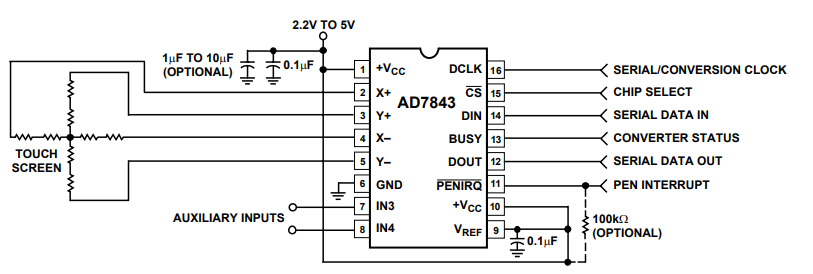
\includegraphics[width=0.8\linewidth]{images/graphic_interface_design/LT24_touchscreen_driver/ad7843_circuit.png}
    \caption{AD7843 connection to the resistive touchscreen.}
    \label{fig:ad7843_circuit}
\end{figure}

From this condition, thanks to some internal switches, the ADC can measure the value of the potential divider, thus obtaining the position of the touched location, as shown in Fig. \ref{fig:ad7843_diff_meas}.

\begin{figure}[!h]
    \centering
    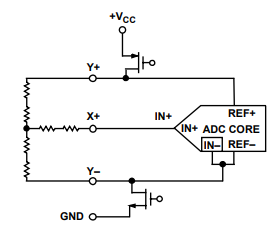
\includegraphics[width=0.6\linewidth]{images/graphic_interface_design/LT24_touchscreen_driver/ad7843_differential_measurement.png}
    \caption{AD7843 Y position measurement in \textit{Differential Reference Mode}.}
    \label{fig:ad7843_diff_meas}
\end{figure}

As we can see, with the \textit{Differential Reference Mode} the analog-to-digital conversion becomes ratiometric and the conversion output is a percentage of the total sheet resistance.

\subsection{Pen Interrupt Request}\label{ref:penirq}
The functional block diagram of the circuit that generates the LT24\_PENIRQ\_N interrupt signal is shown in Fig. \ref{fig:penirq_circuit}.

\begin{figure}[!h]
    \centering
    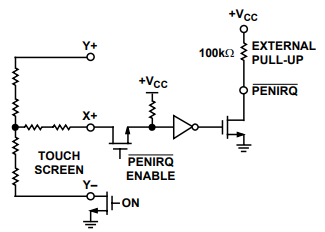
\includegraphics[width=0.5\linewidth]{images/graphic_interface_design/LT24_touchscreen_driver/penirq_circuit.png}
    \caption{$\overline{\text{PENIRQ}}$ functional block diagram.}
    \label{fig:penirq_circuit}
\end{figure}

If the $\overline{\text{PENIRQ}}$ function is enabled, when the touch screen is touched the interrupt output signal (normally high) goes low. Once the START bit is detected, the pen interrupt function is disabled and the $\overline{\text{PENIRQ}}$ cannot respond to screen touches. The $\overline{\text{PENIRQ}}$ output remains low until the fourth falling edge of DCLK after the START bit has been clocked in, at which point it returns high as soon as possible, regardless of the touch screen capacitance. This does not mean that the pen interrupt function is now enabled again because the power-down bits have not yet been loaded to the control register. Regardless of whether $\overline{\text{PENIRQ}}$ is to be enabled again or not, the $\overline{\text{PENIRQ}}$ output normally always idles high. Assuming that the $\overline{\text{PENIRQ}}$ is enabled again, once the conversion is complete, the $\overline{\text{PENIRQ}}$ output responds to a screen touch again. This sequence is illustrated in Fig. \ref{fig:penirq_timing}.

\begin{figure}[!h]
    \centering
    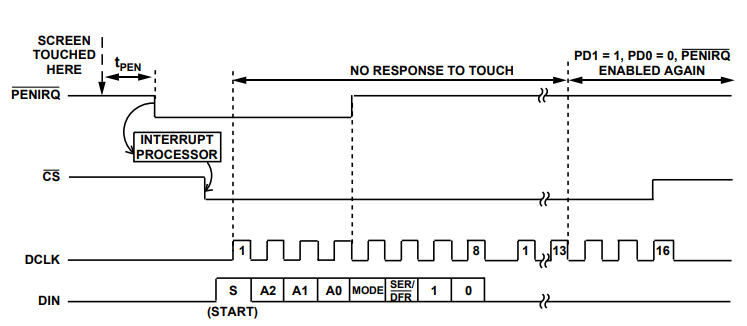
\includegraphics[width=0.8\linewidth]{images/graphic_interface_design/LT24_touchscreen_driver/penirq_timing_diagram.png}
    \caption{$\overline{\text{PENIRQ}}$ timing diagram.}
    \label{fig:penirq_timing}
\end{figure}

\subsection{ADC Interface Synchronization}
From the synchronous design point of view, the interrupt signal is asynchronous and therefore it must be synchronized in order to avoid metastabilities in our system. This is accomplished by means of an \textbf{optimal synchronizer}, shown in Fig. \ref{fig:opt_synch_circuit}.

\begin{figure}[!h]
    \centering
    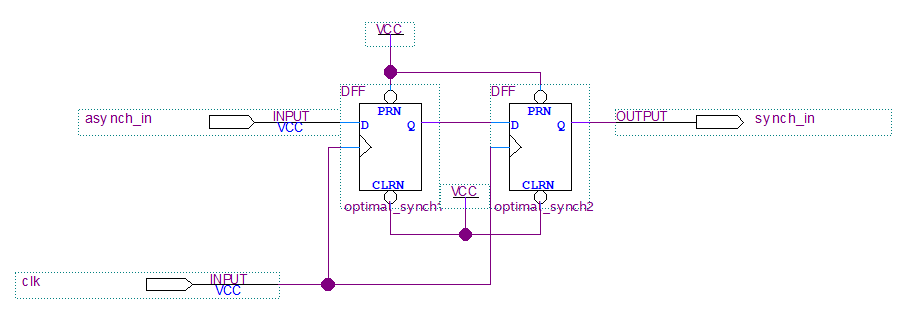
\includegraphics[width=0.8\linewidth]{images/graphic_interface_design/LT24_touchscreen_driver/optimal_synch_circuit.png}
    \caption{Circuit diagram of an optimal synchronizer.}
    \label{fig:opt_synch_circuit}
\end{figure}

However, also the other two input signals, LT24\_ADC\_DOUT and LT24\_ADC\_BUSY, need synchronization: in fact, despite the fact that the ADC clock is generated in the FPGA, it will be certainly affected by some skew, due to both the DCLK generation network (see Sec. \ref{sec:adc_clock}) and the inevitable delay introduce by the PCB routes. Given that LT24\_ADC\_DOUT and LT24\_ADC\_BUSY are synchronous with DCLK, it is necessary to introduce here as well an optimal synchronizer stage. Notice that the optimal synchronizer block is clocked with the global 50 MHz clock, which is approximately 1000 times faster than the change rate of the DOUT signal and approximately 500 times faster than the touchscreen driver operation frequency, therefore it does not introduce a significant delay on this signal.

\subsection{Modelsim Simulation}
This touch screen driver was simulated in Modelsim using a testbench that emulates the behavior of the AD7843. Thanks to this simulation, it was possible to see that the protocol described in the ADC datasheet was fully followed and the conversion outputs are stored in the output registers, as shown in Fig. \ref{fig:touchscreen_simulation}.

\begin{figure}[!ht]
    \centering
    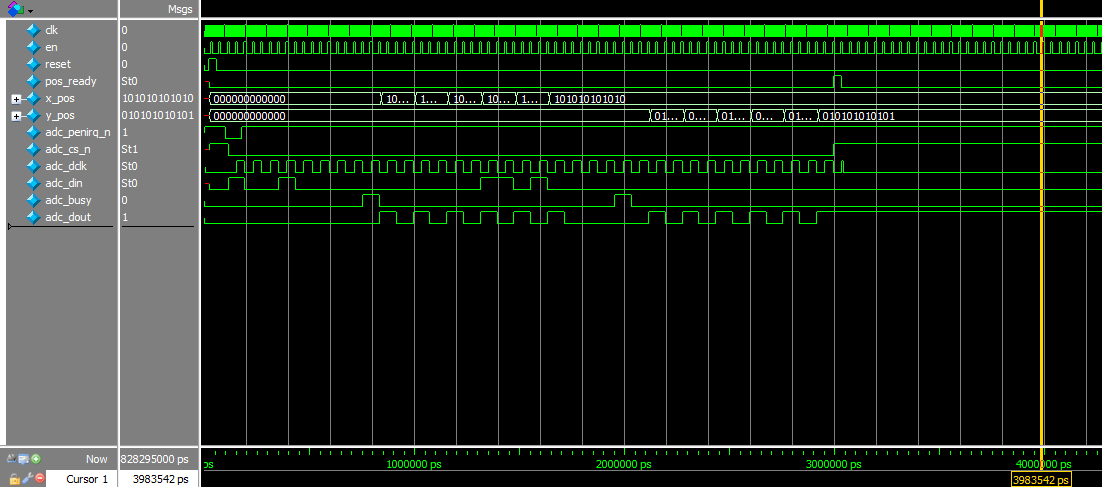
\includegraphics[width=1\linewidth]{images/graphic_interface_design/LT24_touchscreen_driver/touchscreen_simulation.png}
    \caption{LT24 touchscreen driver waveforms simulation in Modelsim.}
    \label{fig:touchscreen_simulation}
\end{figure}

\section{Painter}\label{sec:painter}
The painter represents the interface between the touch screen and the LCD display and it is the only block that has write access to the frame RAM inside the graphic interface sub-system. 

\begin{figure}[!h]
    \centering
    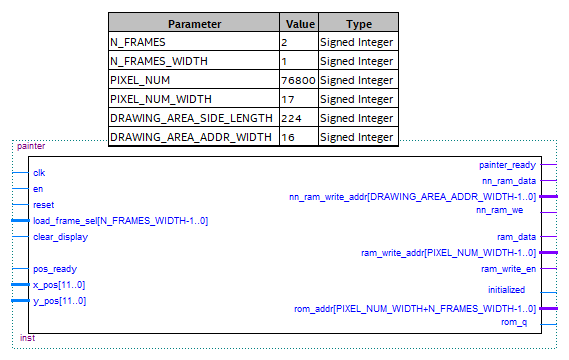
\includegraphics[width=0.8\linewidth]{images/graphic_interface_design/painter/painter_quartus_block.png}
    \caption{Painter Quartus block.}
    \label{fig:painter_quartus_block}
\end{figure}

Upon reset, this module loads a constant frame from a dedicated ROM to the frame RAM: multiple constant frames can be stored inside the frame ROM and the frame with index corresponing to the input \texttt{load\_frame\_sel} value will be loaded. However, in our application only the first constant frame is always selected. The constant frame is loaded also when the \texttt{clear\_display} input is set high or whenever \texttt{load\_frame\_sel} changes.

\begin{figure}[!h]
    \centering
    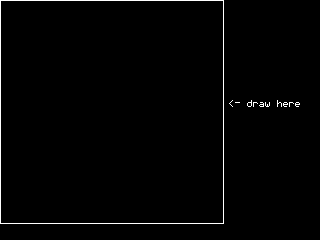
\includegraphics[width=0.5\linewidth]{images/graphic_interface_design/painter/constant_frame.png}
    \caption{Constant frame loaded in the ROM.}
    \label{fig:constant_frame}
\end{figure}

Moreover, the painter monitors its \texttt{pos\_ready} input from the touch screen driver: when high, it reads the \texttt{x\_pos[12:0]} and \texttt{y\_pos[12:0]} inputs, it converts them into coordinates and it writes a white 1-bit pixel at the corresponding memory location in the frame RAM (which will be read by the graphic controller, effectively displaying in real time on the screen what the user draws, see Sec. \ref{sec:graphic_controller}). If the touched location lies inside a certain square area, with side length defined by the parameter DRAWING\_AREA\_SIDE\_LENGTH and with the top left corner aligned with the (0, 0) pixel, a 1 is written inside a specific RAM, used to store the inputs of the neural network. This memory is accessed in the same way as the frame RAM, but it will only have $\text{DRAWING\_AREA\_SIDE\_LENGTH}^2$ 1-bit words. This memory is cleaned whenever a constant frame is loaded to the frame RAM. As shown in figure \ref{fig:constant_frame}, the constant frame loaded helps the user to identify the drawing area that will be used as input of the neural network. In our application, the drawing area has a side length of 224 pixels, so that it is easier for the user to draw inside of it.

\bigskip

The finite-state machine of this system is shown in Fig. \ref{fig:painter_fsm}.

\begin{figure}[!h]
\centering
\resizebox{1\linewidth}{!}{% Reduce size of everything
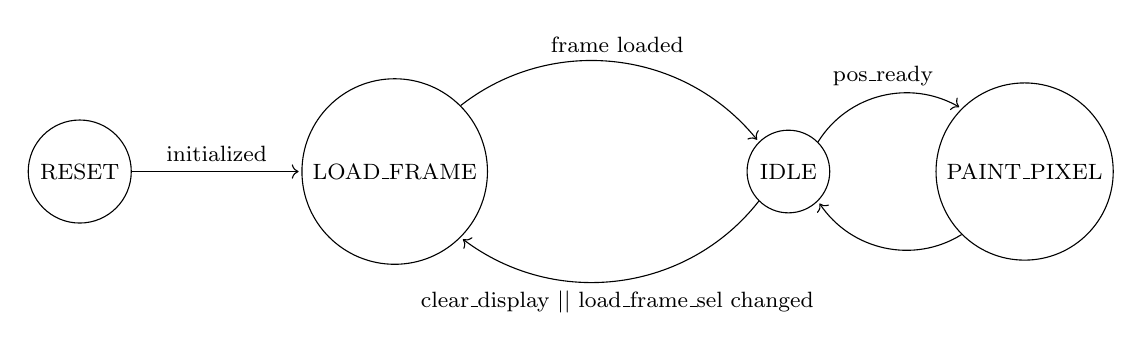
\begin{tikzpicture}[shorten >=1pt, node distance=3cm, on grid,
                    initial distance=1cm, initial text=reset,
                    bend angle=45,
                    every state/.style={font=\footnotesize},
                     initial/.style ={font=\footnotesize}] 
    %\draw[help lines] (0,-5) grid (10,10);

   \node[state,initial] (reset) {RESET};
   \node[state] (load_frame) at (4, 0) {LOAD\_FRAME};
   \node[state] (idle) at (9, 0) {IDLE};
   \node[state] (paint_pixel) [right=of idle] {PAINT\_PIXEL};

   % Define transitions
   \path[->,every node/.style={font=\footnotesize}]
    (reset) edge  node [above] {initialized} (load_frame)
    (load_frame) edge [bend left] node [above] {frame loaded} (idle)
    (idle) edge [bend left] node [above] {pos\_ready} (paint_pixel)
    (idle) edge [bend left] node [below] {clear\_display $||$ load\_frame\_sel changed} (load_frame)
    (paint_pixel) edge [bend left] node [above] {} (idle);
    
\end{tikzpicture}
}
\caption{Painter state flow.}
\label{fig:painter_fsm}
\end{figure}

Notice that the PAINT\_PIXEL requires only one clock cycle to write data to the RAMs.

The following code shows how the input raw data from the ADC is mapped into coordinates values:

\begin{lstlisting}[
language=Verilog,
style=verilog,
caption=Map from the ADC raw data to coordinates.,
label= list:touchscreen_map]
reg [20:0] touchscreen_x_temp;	// Temporary variables for calculations
reg [19:0] touchscreen_y_temp;
wire [8:0] touchscreen_x;	    // Final (x, y) coordinates of touched pixel
wire [7:0] touchscreen_y;
	 
assign touchscreen_x = touchscreen_x_temp[8:0];
assign touchscreen_y = touchscreen_y_temp[7:0]; 
 
// Output ranges from touchscreen ADC
localparam TS_MINX = 12'd0;//750; with 12
localparam TS_MAXX = 12'd4095;
localparam TS_MINY = 12'd0;
localparam TS_MAXY = 12'd4095;// 3750 with 12
 
// Map touchscreen ADC values to pixel coordinates
always @ (*) begin
    if (x_pos < TS_MINX)
        touchscreen_x_temp = 1'b0;
    else if (x_pos > TS_MAXX)
        touchscreen_x_temp = COL_NUM - 1'b1;
    else
        touchscreen_x_temp = ((x_pos - TS_MINX) * (COL_NUM - 1'b1)) >> 12;
           
    if (y_pos < TS_MINY)
        touchscreen_y_temp = ROW_NUM - 1'b1;
    else if (y_pos > TS_MAXY)
        touchscreen_y_temp = 1'b0;
    else
        touchscreen_y_temp = ((TS_MAXY - y_pos) * (ROW_NUM - 1'b1)) >> 12;
end
\end{lstlisting}

As we can see, the raw values, which range from 0 to 4095 (12-bit resolution), is linearly converted into a column and row number, using the following equations:

\begin{equation}
    \texttt{touchscreen\_x}=\frac{\texttt{x\_pos}\times319}{4096}
\end{equation}
\begin{equation}
    \texttt{touchscreen\_y}=\frac{(4095-\texttt{y\_pos})\times239}{4096}
\end{equation}

The equation for the Y coordinate uses the complementary value of \texttt{y\_pos} because of the way the screen is oriented from the user point of view: for the ADC, the Y=0 row is the bottom one (the closest to the LT24 connector), whereas in our application it is the top one (oppsite to the LT24 connector).

\section{Average Pooling}\label{sec:average_pooling}
The average pooling block purpose is to resize the input image contained inside the drawing area and stored in the NN input frame RAM, so that it can be elaborated by the neural network.

\begin{figure}[!h]
    \centering
    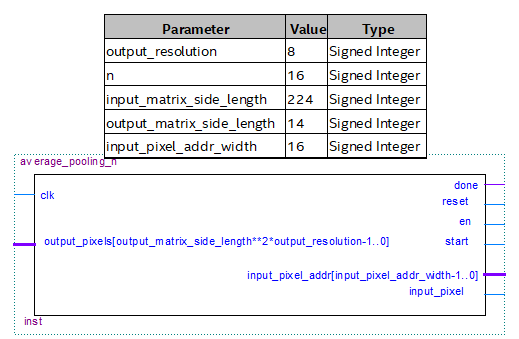
\includegraphics[width=0.75\linewidth]{images/graphic_interface_design/average_pooling/average_pooling_quartus_block.png}
    \caption{Average pooling Quartus block.}
    \label{fig:avg_pooling_quartus_block.}
\end{figure}

As explained in Sec. \ref{sec:painter}, the input image from the painter has a total number of $224^2=50176$ 1-bit pixels. However, as thoroughly explained in Sec. \ref{sec:neural_network_architecture}, the input image should be a 2D matrix of 8-bit signed integer pixels with side length equal to 14. This size reduction is performed through an average pooling operation: it consists in calculating the average value of the pixels inside a sub-matrix with size $n\times n$ and using that value as output pixel; this operation is repeated for all the output pixels, shifting the pool matrix through the input matrix, as shown in Fig. \ref{fig:avg_pooling_operation}.

\begin{figure}[!h]
    \centering
    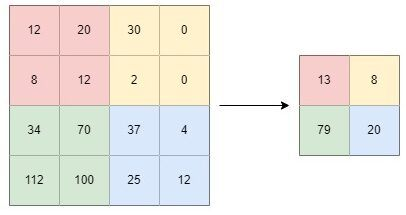
\includegraphics[width=0.8\linewidth]{images/graphic_interface_design/average_pooling/avg_pooling_illustration.png}
    \caption{Average pooling operation.}
    \label{fig:avg_pooling_operation}
\end{figure}

In our case, the size of the average pooling matrix must be of $16\times16$, so that the final dimensions are correct. A total of 196 average operations are necessary so to cover the whole input matrix area.

In order to save resources on the FPGA, the average pooling block has been designed to work in a serial manner, instead of performing a parallel computation of all the outputs:
\begin{itemize}
    \item When a \texttt{start} signal is asserted, the average pooling block starts fetching the values of the pixels inside the first pool (starting from the top left) by interrogating the NN inputs RAM seen before in Sec. \ref{sec:painter}.
    \item Once all the $16^2=256$ 1-bit pixels are fetched and temporarely stored inside local registers, a $n$ pixels averager is activated. In one clock cycle it sums the input pool pixels, it extends the resolution to 8 bit and divides the result by 256.
    \item The output of the $n$ pixels averager is stored in a output buffer, that contains the the output 8-bit resolution matrix.
    \item The next pool is fetched and the steps above are repeated until the end of the NN inputs memory is reached.
\end{itemize}

Notice that the output matrix is presented in a parallel manner to the neural network input, but that is not a concern, because only $14\times14\times8\ \text{bit}=1568\ \text{bit}$ are needed. A real problem for the utilization of the logic elements inside the FPGA would have been carrying all the output bits simultaneously from the painter module to the average pooling module: in that case $224\times224\times1\ \text{bit}=50176\ \text{bit}$ would have been necessary. This serial solution also helps reduce timing issues.

The finite-state machine of this module is shown in Fig. \ref{fig:average_pool_fsm}.

\begin{figure}[!h]
\centering
\resizebox{1\linewidth}{!}{% Reduce size of everything
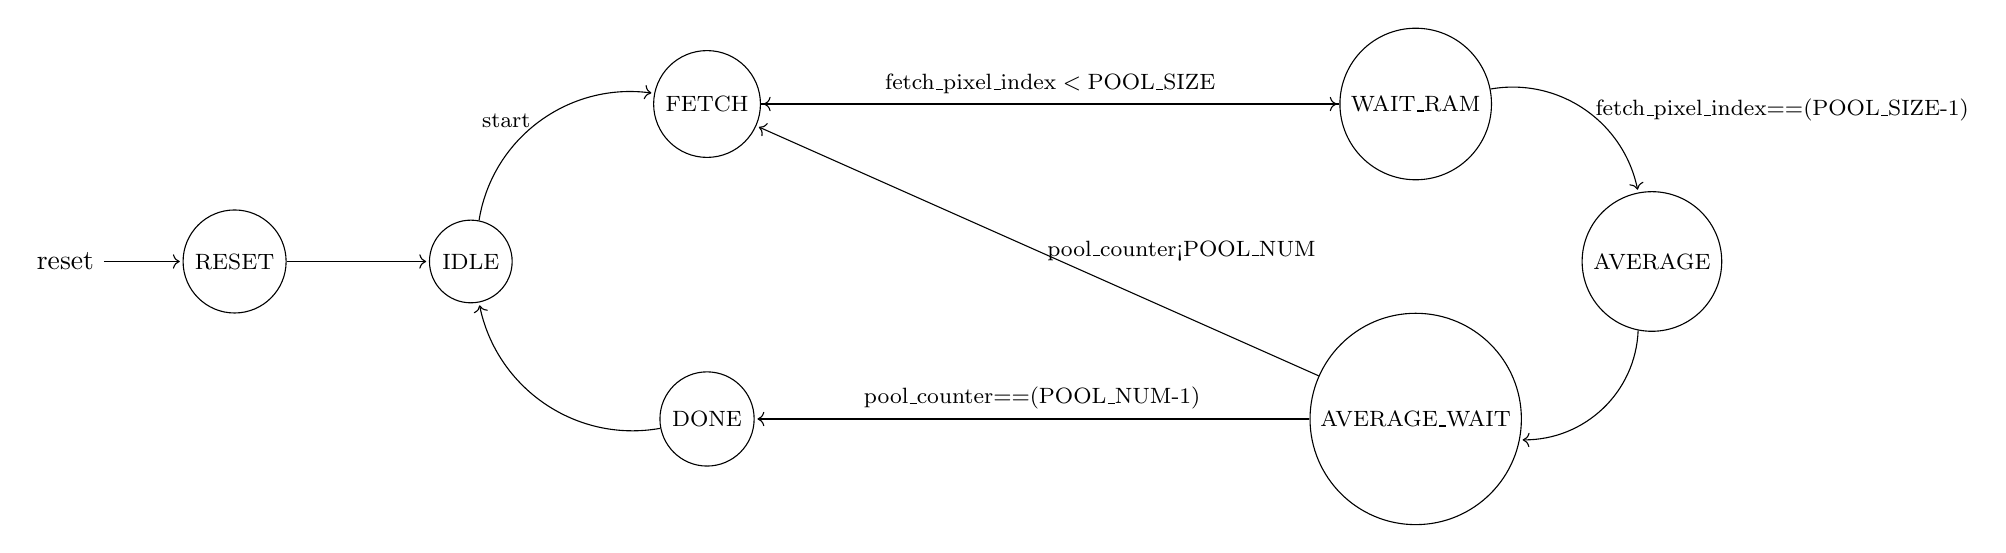
\begin{tikzpicture}[shorten >=1pt, node distance=3cm, on grid,
                    initial distance=1cm, initial text=reset,
                    bend angle=45,
                    every state/.style={font=\footnotesize}]
    %\draw[help lines] (0,-5) grid (10,10);

   \node[state,initial] (reset) {RESET};
   \node[state] (idle) [right=of reset] {IDLE};
   \node[state] (fetch) at (6, 2) {FETCH};
   \node[state] (wait_ram) at (15, 2) {WAIT\_RAM};
   \node[state] (average) at (18, 0) {AVERAGE};
   \node[state] (average_wait) at (15, -2) {AVERAGE\_WAIT};
   \node[state] (done) at (6, -2) {DONE};   

   % Define transitions
   \path[->,every node/.style={font=\footnotesize}]
   (reset) edge node {} (idle)
   (idle) edge [bend left] node [left] {start} (fetch)
   (fetch) edge node [above] {} (wait_ram)
   (wait_ram) edge node [above] {$\text{fetch\_pixel\_index}<\text{POOL\_SIZE}$} (fetch)
   (wait_ram) edge [bend left] node [right] {fetch\_pixel\_index==(POOL\_SIZE-1)} (average)
   (average) edge [bend left] node [below] {} (average_wait)
   (average_wait) edge node [right] {pool\_counter<POOL\_NUM} (fetch)
   (average_wait) edge node [above] {pool\_counter==(POOL\_NUM-1)} (done)
   (done) edge [bend left] node {} (idle);
    
\end{tikzpicture}
}
\caption{Average pooling state flow.}
\label{fig:average_pool_fsm}
\end{figure}
As we can see, two counters are needed, one that keeps track of the current pool \texttt{pool\_counter} and the other that counts the number of pixels fetched inside the current pool \texttt{fetch\_pixel\_index}. Both of these counters are made of two counters, one for the row (e.g the current row inside the pool matrix) and one for the column (e.g. the current column inside the pool matrix). This is necessary to make it easier to compute addresses (one is the address of the current pixel in the NN inputs RAM to be fetched and the other is the address of the current 8-bit pixel in the output register matrix that is being computed): in fact, without this solution integer division operations would have been necessary. The following Verilog code is used to compute the address of the pixel that has to be fetched from the RAM as a function of the current pool and the current element inside the pool:

\begin{lstlisting}[
language=Verilog,
style=verilog,
caption=Fetch pixel address calculation.,
label= list:fetch_addr_calc]
// Assign the address of the current pixel to be fetched
reg [input_pixel_addr_width-1:0] top_left_pixel_addr;
always @ (*) begin
    top_left_pixel_addr = output_col_counter * n + output_row_counter * n * input_matrix_side_length;
    input_pixel_addr = top_left_pixel_addr + pool_col_counter + pool_row_counter * input_matrix_side_length;
end
\end{lstlisting}
where \texttt{top\_left\_pixel\_addr} is the address inside RAM of the top left pixel of the current pool matrix.

\subsection{Average n Pixels}
This module computes the average value between $n$ pixels with resolution 1-bit. The output resolution can be set through a parameter and in our case is equal to 8.

As explained before, this module sums all the 1-bit input pixels and divides this value by the number of input pixels. In order to avoid timing issues, the number of pixels $n^2$ can only be a power of 2, so that the division will result in a bit shift to the right. Since the output will be interpreted by the neural network as a signed 8-bit integer and all the pixels are positive by definition, the output pixel value will range between 0 and $2^{\texttt{output\_resolution-1}}-1=127$. The Verilog code that performs this conversion is shown in the following:

\begin{lstlisting}[
language=Verilog,
style=verilog,
caption=Average n pixels code.,
label= list:average_n_pixels_code]
// Declare sum with enough bits to contain the sum of n integers of resolution bits
reg [1+$clog2(n):0] sum;

integer i;
always @ (*) begin
    sum = 0;
    for (i = 0; i < n; i = i + 1)
        sum = sum + input_pixels[i +: 1];
end

// Temporary registred output for calculations
reg [$clog2(n)+output_resolution-1:0] out_temp;
   
// Clear or update data
always @ (posedge clk) begin
	if (reset)
		out_temp <= 0;
	else
        out_temp <= (sum * ((1'b1<<(output_resolution - 1'b1)) - 1'b1)) >> $clog2(n);
end
	
// Assign only output_resolution LSBs to out
assign out = out_temp[output_resolution-1:0];
\end{lstlisting}
Note that the calculation is performed in 1 clock cycle.

\chapter{FPGA Implementation}
The previously designed system has been implemented on a 10M50DAF484C7G MAX10 FPGA, mounted on the DE10-Lite development board.
\section{Pin Assignments}
All the pins have been assigned to the their respecitve I/O pin, as specified in the \href{https://ftp.intel.com/Public/Pub/fpgaup/pub/Intel_Material/Boards/DE10-Lite/DE10_Lite_User_Manual.pdf}{manual} of the DE10-Lite board. Their I/O standard is set to 3.3V LVTTL.

\section{Resource Utilization}

The resources used on the MAX10 by the final design are shown in Table \ref{tab:res_utilization}.

\begin{table}[!h]
\renewcommand{\arraystretch}{1.5}
\centering
\begin{tabular}{|c|c|c|c|}
\hline
\textbf{Resource}         & \textbf{Used} & \textbf{Available} & \textbf{Percentage} \\ \hline
Logic elements            & 17281         & 49760              & 35\%                \\ \hline
I/O pins                  & 39            & 360                & 11\%                \\ \hline
Memory bits               & 327680        & 1677312            & 20\%                \\ \hline
Embedded multiplier 9-bit & 62            & 288                & 22\%                \\ \hline
PLLs                      & 0             & 4                  & 0\%                 \\ \hline
UFM blocks                & 0             & 1                  & 0\%                 \\ \hline
ADC blocks                & 0             & 2                  & 0\%                 \\ \hline
\end{tabular}
\caption{Total design resource utilization.}
\label{tab:res_utilization}
\end{table}

These utilization percentages are low enough to guarantee the success of the fitting tool. However, previous versions of the system had much higher resource utilization percentages, which could not be fitted on our hardware. For this reason, the following design choices had to be made:
\begin{itemize}
    \item The resolution of the pixels stored in the frame RAM had to be reduced to 1 bit to avoid using all the available memory bits.
    \item The interface between the average pooling and the graphic modules had to be serialized with the use of a RAM to reduce the number of logic elements previously used to simultaneously transfer the pixels inside the drawing area and compute the average value (full adders).
    \item The number of layers of the neural network had to be optimized, in order to reduce the number of used embedded multipliers.
\end{itemize}

\section{Timing Analysis}
The timing analysis was run in the worst process corner of a slow model with a 1200 mV power supply at 85°C. The constraint on the clock (50 MHz, 50\% duty cycle) was set through the following TCL script:

\begin{lstlisting}[
style=tclstyle,
caption=TCL clock constraint.
]
#**************************************************************
# Time Information
#**************************************************************

set_time_format -unit ns -decimal_places 3



#**************************************************************
# Create Clock
#**************************************************************

create_clock -name {clk_50} -period 20.000 -waveform { 0.000 10.000 } [get_ports {MAX10_CLK1_50}]
\end{lstlisting}

The obtained results are the following:

\begin{table}[!h]
\renewcommand{\arraystretch}{1.5}
\centering
\begin{tabular}{|c|c|}
\hline
\textbf{Setup slack} & \textbf{Maximum clock frequency} \\ \hline
0.695 ns             & 51.8 MHz     \\ \hline
\end{tabular}
\caption{Timing analysis results in the worst process corner.}
\label{tab:timing_analysis}
\end{table}

As we can see from the report on the critical paths present in our design, shown in Fig. \ref{fig:report_path}, the paths with the most delay are the ones associated to the combinatorial network that computes the sum of the pixels inside the module that averages the pixels of the pool matrix. In order to improve the setup slack time, one possible future improvement could be to break that critical path using a pipelining technique.

\begin{figure}[!h]
    \centering
    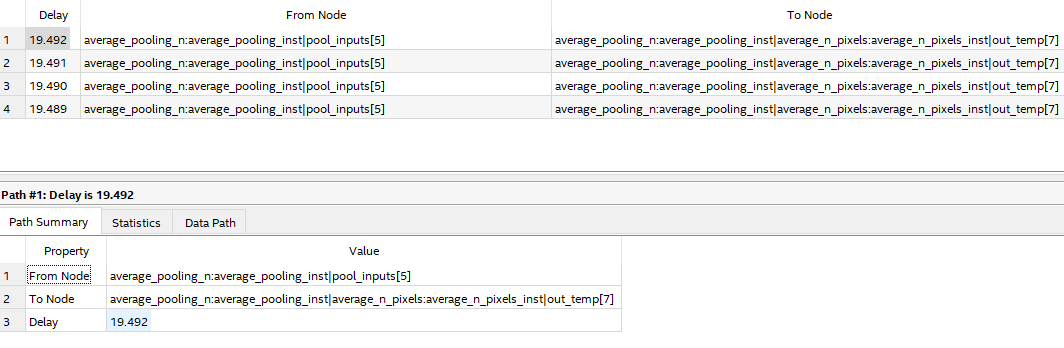
\includegraphics[width=1\linewidth]{images/fpga_implementation/report_path.png}
    \caption{Timing analyzer critical path report.}
    \label{fig:report_path}
\end{figure}

\section{Warnings}
In Fig. \ref{fig:analysis_synth_warnings} the warnings returned by the Analysis \& Synthesis tool:

\begin{figure}[!h]
    \centering
    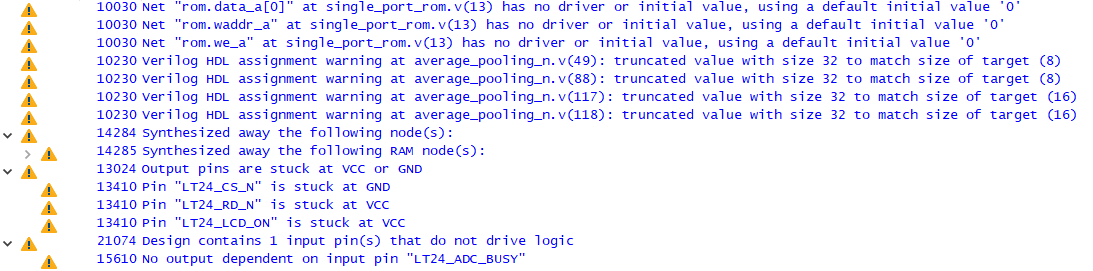
\includegraphics[width=1\linewidth]{images/fpga_implementation/warnings_synth.png}
    \caption{Analysis \& Synthesis warnings.}
    \label{fig:analysis_synth_warnings}
\end{figure}

\begin{itemize}
    \item The first three warnings concern the frame ROM, where an \texttt{initial} structure is used to initialize the memory. However, these warnings do not result in any initialization problem, because the constant frame is loaded with no issues.
    \item The following four messages warn about truncation of variables in the average pooling module. These are due to the fact that these variables are actually module parameters of type integer (32 bit). However, these warnings were predictable and these variables' values are accurately chosen so that the assignment expression always fits inside the target of the assignment.
    \item The following warning concerns the frame ROM. A part of it is synthesized away because it is actually never accessed. This fact is known and it does not represent a problem, because, even though the constant frame selection feature was implemented in the painter module, in the final design it is not used and the \texttt{load\_frame\_sel} selector is tied to GND on purpose. This way only the first frame is selected and the second one is never reached.
    \item The LT24\_CS\_N chip select is kept always at GND (active) because there was no need to disable it, as we had only one ILI9341 LCD controller on the same parallel 8080-I bus. The LT24\_RD\_N pin is always high (disabled) because in this design there was no need to read data from the ILI9341. The LT24\_LCD\_ON pin is always high (enabled) so that the LCD backlight is always turned on.
    \item The LT24\_ADC\_BUSY does not drive any logic in the touchscreen driver, because, as declared in the AD7843 datasheet, that pin is enabled during the acquisition phase of the ADC for exactly one ADC clock (DCLK) cycle. Therefore, the touchscreen driver finite-state machine simply waits for one DCLK cycle, independently from the value of the  LT24\_ADC\_BUSY input. 
\end{itemize}

\bigskip

The fitter does not return any particular warning. It only reminds that the I/O pins must meet the Intel FPGA requirements for 3.3-, 3.0- and 2.5-V interfaces.

\bigskip

For what concerns the timing analyzer, it warns of the lack of clock uncertainty assignments: however, this level of accuracy in the clock model is beyond the scope of this project. Moreover, it warns of the lack of constraints on the I/O port used: these could be defined for a better analysis of the behavior at these ports, however, they can be ignored.

\chapter{Future Improvements}

One of the key areas for future improvement in this project is the on-board implementation of backpropagation, allowing the system to perform real-time training and adaptation without relying on external computation. Currently, the neural network used for digit recognition is pre-trained, and only inference is executed on the FPGA. Implementing backpropagation would enable the system to learn directly from user input, making it adaptable to different handwriting styles over time.  

Backpropagation is a computationally intensive process that involves multiple steps, including forward propagation, where the input is processed through the neural network using current weight values, and error calculation, where the predicted output is compared to the actual label. This is followed by gradient computation, which determines how each weight contributes to the error, and weight updating, where the gradient descent algorithm is used to adjust the weights accordingly.  

One crucial aspect of implementing on-board training is the need for non-volatile memory to store updated weights between power cycles. Since the FPGA’s internal registers and memory elements are volatile, external storage is required to maintain learning progress. One possible solution is to use an external SD card, which provides high storage capacity and flexibility. Alternatively, an EEPROM could be used as a more energy-efficient storage option, or, if available, on-chip Flash memory could reduce data transfer overhead and improve system responsiveness.  

Beyond backpropagation, other improvements could enhance the system’s performance and usability. Increasing the complexity of the neural network, for example, by adding more layers or neurons, could improve classification accuracy at the cost of additional computational requirements. Implementing quantization techniques could help reduce power consumption while maintaining recognition performance. Additionally, integrating support for multiple handwriting styles by collecting and fine-tuning user-specific training data would allow the model to be more versatile and adaptive.  

By incorporating these improvements, the project could evolve into a fully autonomous edge-learning system capable of real-time adaptation and continuous learning, further enhancing its usability and making it a more practical solution for real-world applications.  


\chapter{Conclusions}

\begin{figure}[!h]
    \centering
    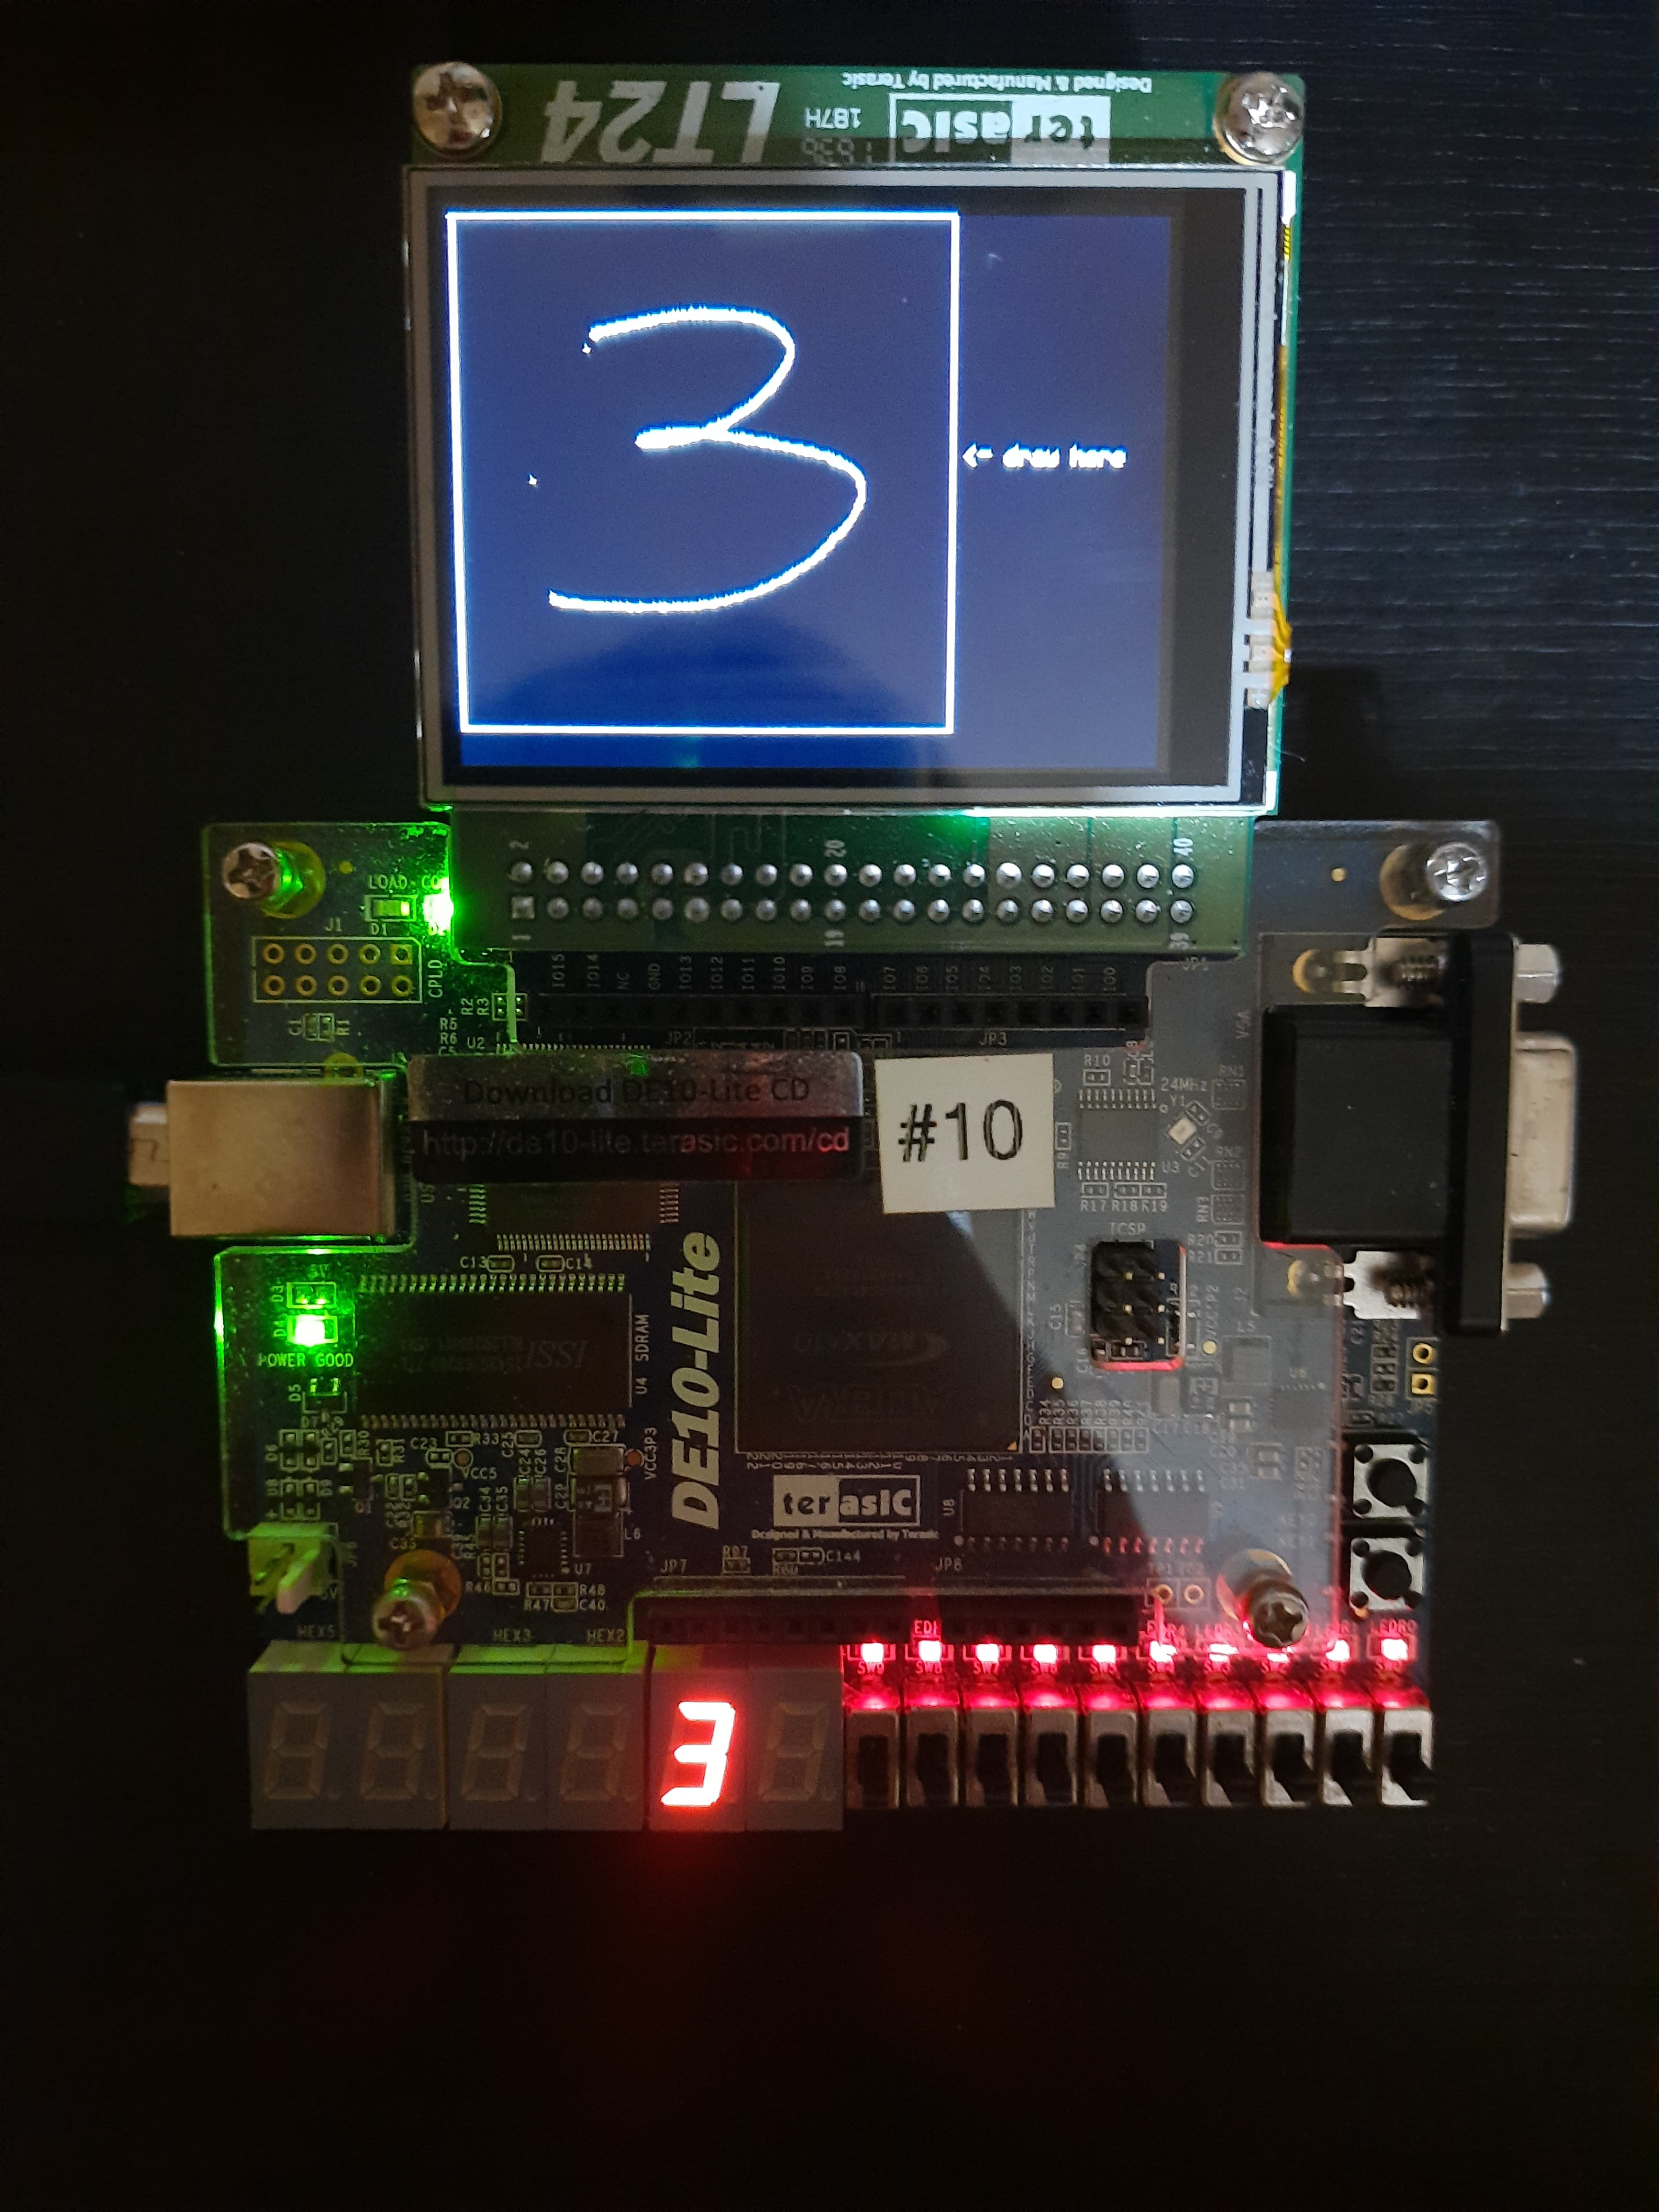
\includegraphics[width=0.5\linewidth]{images/conclusions/test.jpg}
    \caption{Handwritten digit recognition design loaded on the DE10-Lite MAX10 FPGA board.}
    \label{fig:test}
\end{figure}

This project successfully demonstrated the implementation of a \textbf{handwritten digit recognition system} using a \textbf{touchscreen interface} and an \textbf{FPGA-based design} as shown in fig \ref{fig:test}. The complete system was deployed on the \textbf{Altera DE10-Lite} development board, featuring a \textbf{MAX10 FPGA}. The LT24 touchscreen was used for user input, while the recognized digit was displayed on a seven-segment display. Additionally, push buttons were integrated to facilitate user interaction.  

The project adhered to the fundamental principles of digital design, following a structured workflow that included \textbf{design}, \textbf{hardware implementation in Verilog}, functional verification and simulation using Quartus Prime and ModelSim, as well as timing analysis and fitting considerations. Finally, the system was tested on real hardware using Quartus, validating its correct functionality.  

The final implementation aligned well with expectations, demonstrating that AI on the edge is a feasible and efficient alternative. This project highlights how a dedicated hardware design can deliver high performance and reliability for embedded AI applications. Future work could focus on optimizing resource utilization, improving classification accuracy, or extending the system to support more complex neural networks. 

\printbibliography 


\end{document}